\documentclass[a4paper, 12pt, oneside]{book}

\usepackage[utf8]{inputenc}
\usepackage{lmodern}
\usepackage{layout}
\usepackage{emptypage}
\usepackage{fancyhdr}
\usepackage[spanish,es-tabla]{babel}
%\usepackage[Conny]{fncychap}
%\usepackage{graphicx}
\usepackage{subfigure} % subfiguras
\usepackage{caption}
\usepackage{mathtools}
\usepackage{hyperref}
\usepackage[a4paper,top=3cm, bottom=3cm, inner=2.5cm, outer=2.5cm]{geometry}
\usepackage{listings}
\usepackage[spanish]{babel}
\usepackage{url}
\usepackage{float}
\usepackage{multirow}
\usepackage{rotating} 
\usepackage{color}
\usepackage{colortbl}
\usepackage[table]{xcolor}
\usepackage[spanish]{babel}
\usepackage{enumerate}
\usepackage[acronym, nonumberlist]{glossaries}
\makeglossaries
\newacronym{stem}{STEM}{Science, Technology, Engineering and Math}
\newacronym{gui}{GUI}{Graphical User Interface}
\newacronym{sdf}{SDF}{Simulation Description Format}
\newacronym{xml}{XML}{Extensible Markup Language}
\newacronym{api}{API}{Application Programming Interface}
\newacronym{ice}{ICE}{Internet Communications Engine}
\newacronym{slam}{SLAM}{Simultaneous Localization and Mapping}
\newacronym{ros}{ROS}{Robot Operating System}

\makeatletter
\renewcommand{\@makeschapterhead}[1]{%
%  \vspace*{50\p@}%
  \vspace*{0\p@}%
  {\parindent \z@ \raggedright
    \normalfont
    \interlinepenalty\@M
    \Huge \bfseries  #1\par \nobreak
%    \vskip 40\p@
    \vskip 15\p@
  }}
\makeatother

\renewcommand{\baselinestretch}{1.4}
\setlength{\headheight}{16pt} 
\captionsetup{justification=justified}
\pretolerance=1000

\chead[]{}
\rhead[]{}
\renewcommand{\headrulewidth}{0.5pt}

\pagestyle{empty}

\title{Nuevas Prácticas en el Entorno Docente de Robótica JdeRobot-Academy}
\author{Irene Lope Rodríguez}

\lstset{
	float=hbp,
	basicstyle=\ttfamily\small,
	columns=flexible,
	tabsize=4,
	frame=single,
	extendedchars=true,
	showspaces=false,
	showstringspaces=false,
	numbers=none,
	numberstyle=\tiny,
	breaklines=false,
	breakautoindent=true,
	captionpos=b
}
\setcounter{tocdepth}{4}
\setcounter{secnumdepth}{4}

\definecolor{lightgray}{gray}{0.9}

\begin{document}
%%%%%%%%%%%%%%% Portada %%%%%%%%%%%%%%%%%%%%
\begin{titlepage}
	\begin{center}
		\vspace*{3mm}
		\begin{center}
			
\includegraphics[width=0.4\linewidth]{figures/logo.jpg}
		\end{center}
		\vspace{6.5mm}
		
		\fontsize{15.5}{14}\selectfont ESCUELA TÉCNICA SUPERIOR DE INGENIERÍA DE TELECOMUNICACIÓN
		\vspace{13mm}
		
		\fontsize{14}{14}\selectfont GRADO EN INGENIERÍA EN SISTEMAS \\ AUDIOVISUALES Y MULTIMEDIA
		
		\vspace{70pt}
		
		\fontfamily{lmss}\fontsize{15.7}{14}\selectfont \textbf{TRABAJO FIN DE GRADO} 
		
		\vspace{25mm}
		\begin{huge}
			Nuevas Prácticas en el Entorno \\ \vspace{0.4cm} Docente de Robótica JdeRobot-Academy
		\end{huge}
		
		\vspace{25mm}
		
		\begin{large}
			Autora: Irene Lope Rodríguez
			
			Tutor: José María Cañas Plaza
			
			\vspace{10mm}
		\end{large}
		\begin{normalsize}
			Curso académico 2017/2018		
		\end{normalsize}
		\vspace{10mm}
		
	\end{center}
	
\end{titlepage}




\pagenumbering{Roman}

%%%%%%%%%%%%%%% Agradecimientos %%%%%%%%%%%%
\chapter*{Agradecimientos}
En primer lugar, quiero darle las gracias a mi familia por todo su interés y apoyo. En especial a mis padres, por estar a mi lado en todo momento, apoyarme en todas mis decisiones y darme todo su cariño. Gracias por todo lo que habéis hecho por mi a lo largo de toda mi vida.\\

También, quería agradecer a mi tutor José María la oportunidad de realizar este proyecto así como toda su ayuda, dedicación e interés durante los meses de desarrollo del trabajo.\\

Por otro lado, me gustaría darle las gracias a mi compañera proyecto Vanessa por toda su ayuda y ánimo cuando las cosas parecían que no salían y por ser un gran apoyo en estos meses de trabajo. Además, quería darle las gracias a mis compañeros de laboratorio, en especial a Fran por su infinita ayuda, a Aitor por sacarnos de más de un atasco y por su puesto, a Nacho y Carlos por los buenos ratos que nos han hecho pasar.\\

Muchas gracias a mis amigos, a los de siempre: Ayrton, Emilio, Ana, Jumana, y en especial a mi mejor amigo Pablo, por animarme cuando más lo necesitaba, por hacerme reír cada día y por seguir a mi lado durante tantos años. Y no me puedo olvidar de mis amigas de la universidad: Carol, María, Chris y Natalia, por hacer que las clases fueran menos duras y las horas de estudio más divertidas.\\

Y por último, mi más sincero agradecimiento a una de las personas más importantes de mi vida, a mi pareja Carlos, porque sin él, habría tirado la toalla hace mucho tiempo. Simplemente, gracias por todo.

\begin{flushright}
	\emph{¡Muchas gracias a todos!}
\end{flushright}


%%%%%%%%%%%%%%% Resumen %%%%%%%%%%%%%%%%%%%%
\chapter*{Resumen}

La robótica es una rama de la ingeniería que emplea la informática para diseñar y desarrollar sistemas y máquinas que faciliten la vida del ser humano, e incluso sustituirle en determinadas tareas. Se pueden encontrar robots en diferentes áreas y entornos como la industria, la automovilística, la medicina o la domótica, entre otros. Debido a que actualmente la robótica está en continua expansión, es necesario formar a personas para que sean capaces de programar estos robots. \\

El objetivo de este proyecto es la creación de dos nuevas prácticas en el entorno educativo JdeRobot-Academy. Estas prácticas están programadas en el lenguaje Python y se ha hecho uso del simulador Gazebo para realizar las distintas pruebas hasta conseguir un resultado final satisfactorio. También se ha utilizado la librería OpenCV para el tratamiento digital de las imágenes y la herramienta PyQt5 para el desarrollo de la interfaz gráfica de cada una de las prácticas.\\

La primera práctica, llamada \textit{``Coche autónomo negocia un cruce''}, trata de conseguir que un coche autónomo negocie con éxito un cruce. Primero, que sea capaz de reconocer una señal de STOP. Una vez detecte la señal, el coche tendrá que frenar en un cruce y detectar si hay otros coches circulando por la carretera. En el caso de que no aparezcan coches, deberá realizar un giro a la izquierda o a la derecha y continuar su camino. Para ello, se utilizarán tres cámaras de vídeo instaladas en el robot (una en el techo y dos en los faros del coche). \\

La segunda práctica, \textit{``Aspiradora autónoma con autolocalización''}, consiste en que una aspiradora autónoma barra la mayor superficie posible de un apartamento. Dicha aspiradora posee el mapa de la casa y tiene instalado un sistema de autolocalización que le permite saber en todo momento cual es su ubicación en el mundo.



\cleardoublepage

%%%%%%%%%%%%%%% Índices %%%%%%%%%%%%%%%%%%%%
%\cleardoublepage
\renewcommand{\tablename}{Tabla}
%\renewcommand{\listtablename}{Índice de tablas}
%\tableofcontents

%\cleardoublepage % Í­ndice de figuras
%\addcontentsline{toc}{chapter}{\listfigurename}
%\listoffigures

%\cleardoublepage % Í­ndice de tablas
%\addcontentsline{toc}{chapter}{Índice de tablas}
%\listoftables 
\cleardoublepage
\tableofcontents % indice de contenidos

\cleardoublepage
\listoffigures % indice de figuras
\addcontentsline{toc}{chapter}{Índice de figuras} % para que aparezca en el indice de contenidos

\cleardoublepage
\listoftables % indice de tablas
\addcontentsline{toc}{chapter}{Índice de tablas} % para que aparezca en el indice de contenidos


%%%%%%%%%%%%%%% Acronimos %%%%%%%%%%%%%%%%%%%%

\renewcommand{\acronymname}{Acrónimos}
\cleardoublepage
\printglossary[type=\acronymtype]
\addcontentsline{toc}{chapter}{Acrónimos}
\cleardoublepage
 
%%%%%%%%%%%%%%% Capí­tulos %%%%%%%%%%%%%%%%%%
\pagestyle{fancy}
\pagenumbering{arabic}
\setlength{\parindent}{6mm}

\lhead[]{CAPÍTULO \thechapter. INTRODUCCIÓN}
\chapter{Introducción}\label{cap.introduccion}
En este capítulo se definirá el contexto en el cual se sitúa este proyecto así como la motivación principal que ha llevado a desarrollarlo. Se explicará de forma general qué es la robótica, sus aplicaciones y algunos softwares utilizados para la programación de robots. También se expondrá su uso en docencia hoy en día y se comentará de manera general la plataforma JdeRobot-Academy.

\section{Robótica}
La robótica es una rama de la ingeniería que emplea la informática para diseñar y desarrollar sistemas que permitan facilitar la vida del ser humano, e incluso sustituirle en determinadas tareas. Esta rama usa conceptos de diversas disciplinas, tales como la física, las matemáticas, la electrónica, la mecánica, la inteligencia artificial o la ingeniería de control. Mediante todas estas disciplinas realiza diversas máquinas que ejecutan diferentes comportamientos en función de su propósito. Estas máquinas se denominan ``robots''. En el futuro, dominar esta disciplina será clave debido a que cada vez de forma más habitual se implantan robots en diferentes empleos, como pueden ser las cadenas de automatización. \\

\subsection{Historia de la robótica}
El término ``robot'', viene de la palabra checa ``robota'', cuyo significado es ``trabajo forzado''. Dicha palabra fue introducida por primera vez por el dramaturgo y autor checoslovaco Karel Capek (1890 – 1938), en su obra de teatro R.U.R (Robots Universales de Rossum) en 1921. Con este libro surgió la palabra ``robótica'', pero entonces era un término de ciencia ficción. En base a este término se puede decir que un robot es una máquina programada para moverse, manipular objetos y realizar trabajos, para lo cual debe interaccionar con el entorno que le rodea.\\

Unos años más tarde Isaac Asimov (1920 – 1992) introdujo conceptos acerca de la robótica. Isaac Asimov era un escritor y bioquímico estadounidense nacido en Rusia, el cual publicó el libro ``Yo Robot'' en 1950. Este libro contenía tres leyes de la robótica:

\begin{enumerate}[1.]
    \item Un robot no puede lastimar a un ser humano o permanecer inactivo ante un daño que se le pueda hacer.
    \item El robot debe obedecer al ser humano excepto si contradice la primera ley.
    \item El robot debe proteger su existencia salvo que entre en conflicto con las leyes anteriores.
\end{enumerate}

Con este libro, Isaac Asimov consiguió que la robótica se hiciera popular. Sin embargo, no fue hasta mediados de siglo cuando los robots empezaron a disponer de un sistema de control propio. Hasta entonces eran controlados por seres humanos. \\

En los años 50, los primeros robots móviles fueron construidos por Grey Walter (1910 – 1977). Estos robots eran conocidos como tortugas de Bristol y empleaban válvulas, sensores de luz y detectores de contacto, capaces de evitar obstáculos. También, George Devol (1912 – 2011) patentó el primer robot programable y creó la primera empresa dedicada a la robótica llamada Unimation (Universal Automation) junto con Josef Engelberger (1925 - 2015). \\

En la década de los 70, se desarrolló el robot JPL Rover en la Jet Propulsion Laboratory en Pasadena. Su principal fin era la exploración espacial empleando una cámara de televisión, un láser de telemetría y sensores táctiles. Además, Hans Moravec (1948) diseñó CART en Stanford. Este robot evitaba obstáculos mediante una cámara. Para ello creaba un modelo bidimensional de su alrededor a partir de nueve fotos tomadas del entorno. \\

En los años 80, en la Universidad de Stanford, surgen robots capaces de procesar dos cámaras estéreo. Estos robots son capaces de realizar una reconstrucción 3D. 
En el año 2000, Honda lanza el robot Asimo. Este humanoide pretende ayudar a las personas que carecen de movilidad completa, así como animar a la juventud para estudiar ciencias y matemáticas.\\

\begin{figure}[H]
  \begin{center}
    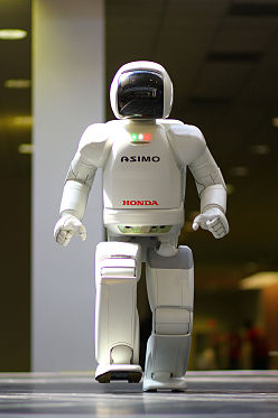
\includegraphics[width=0.2\textwidth]{figures/Introduccion/asimo.png}
		\caption{Robot Asimo}
		\label{fig.asimo}
		\end{center}
\end{figure}

\subsection{Aplicaciones de la robótica}
Actualmente la robótica está en continua expansión. Se pueden encontrar robots en diferentes áreas y entornos. Una de las principales áreas donde se encuentran robots es en la industria. Gracias a los robots se pueden elaborar tareas peligrosas y complejas. El robot industrial, debido a su naturaleza multifuncional puede llevar a cabo un gran número de tareas, totalmente inalcanzable si la mano de obra es humana de manera que se abarata mucho el coste de producción. \\

En el mundo del automóvil se han introducido robots tanto para su construcción, utilizando brazos mecánicos en las cadenas de montaje, como para lograr que los coches sean autónomos. Una de las empresas pioneras en este ámbito es Google que junto con Fiat-Chrysler han desarrollado el proyecto ``Waymo''. Estos vehículos autónomos tienen sensores y software diseñado para detectar personas, ciclistas, vehículos, ciclistas y carreteras a una distancia mayor que dos campos de fútbol en todas las direcciones. \\

\begin{figure}[H]
  \begin{center}
    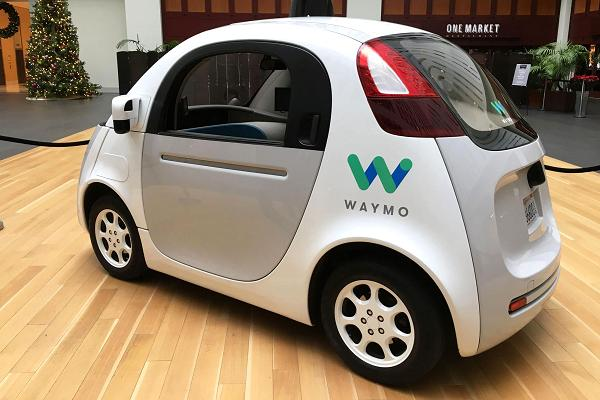
\includegraphics[width=0.4\textwidth]{figures/Introduccion/waymo.jpg}
		\caption{Coche autónomo Waymo}
		\label{fig.waymo}
		\end{center}
\end{figure}

La empresa Tesla también ha desarrollado coches autónomos. Sus coches tienen instaladas ocho que ofrecen una visión de 360 grados alrededor del vehículo en un área de hasta 250 metros. Además, dispone de doce sensores ultrasónicos capaces de detectar objetos de todo tipo y tamaño alrededor del coche, y de un radar delantero que ofrece datos adicionales.

\begin{figure}[H]
  \begin{center}
    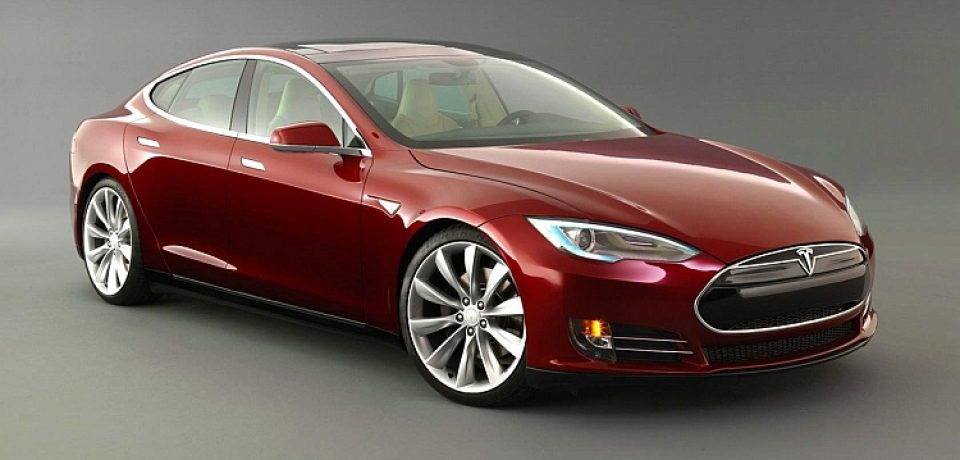
\includegraphics[width=0.4\textwidth]{figures/Introduccion/tesla.jpg}
		\caption{Coche autónomo Tesla (Model S)}
		\label{fig.tesla}
		\end{center}
\end{figure}

El objetivo de los coches autónomos es evitar los accidentes de tráfico y disminuir los atascos. \\

Hoy en día también se pueden encontrar robots en los hogares de las personas, como por ejemplo con aspiradoras autónomas. Estas aspiradoras mediante sensores y el desarrollo de tecnologías en ámbitos como el diseño de mapas y de sistemas de navegación son capaces de limpiar las casas de una manera fiable y robusta ante distintos tipos de obstáculos como muebles o escaleras. La empresa iRobot es pionera mundial en este sector de la robótica con su aspiradora Roomba, aunque también se pueden encontrar otras aspiradoras potentes en el mercado como el robot aspirador Dyson que calcula un patrón de sistema sistemático y de esa forma sabe por dónde ha pasado y dónde tiene que ir a limpiar.\\

\begin{figure}[H]
  \begin{center}
    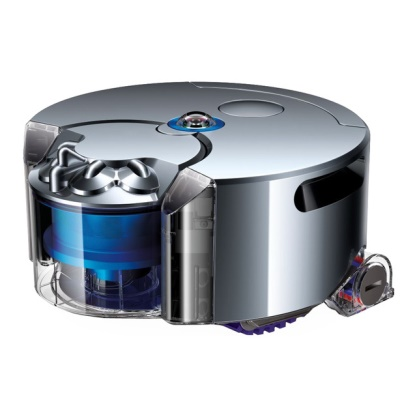
\includegraphics[width=0.3\textwidth]{figures/Introduccion/dyson.jpg}
		\caption{Robot aspirador Dyson}
		\label{fig.dyson}
		\end{center}
\end{figure}

Amazon, en sus almacenes, también ha introducido robots para que la logística sea mucho más rápida y eficaz. Utiliza la automatización para almacenar y retirar los productos. Sus robots son capaces de cargar hasta 1300 Kg y mediante el uso de un láser y una cámara en la parte delantera, son capaces de detectar obstáculos. Se mueven a 1,7 metros por segundo y realizan un pedido en 15 minutos en vez de en 70, disminuyendo así el tiempo de entrega de sus productos.

\begin{figure}[H]
  \begin{center}
    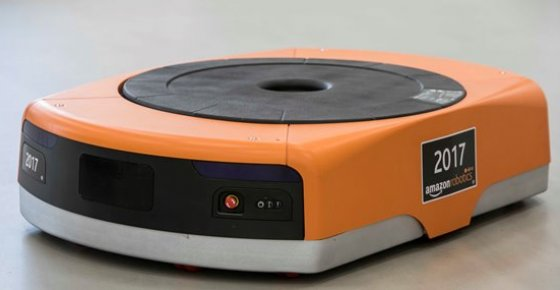
\includegraphics[width=0.3\textwidth]{figures/Introduccion/amazon.jpg}
		\caption{Robot de Amazon Drive}
		\label{fig.amazon}
		\end{center}
\end{figure}

También se pueden encontrar robots en otra gran variedad de ámbitos como en laboratorios de investigación, en la medicina, en el ejército, etc. 

\subsection{Clasificación de robots} 
En función al software desarrollado en el controlador, al diseño mecánico y a la capacidad de los sensores, los robots pueden clasificarse de acuerdo a su arquitectura, su aplicación, su nivel de inteligencia, su generación, su nivel de control y su nivel de lenguaje de programación.

\begin{itemize}
    \item Según su cronología:
    \begin{itemize}
         \item Primera generación: En este grupo se engloban sistemas mecánicos multifuncionales que poseen un sistema de control manual, de secuencia fija o de secuencia variable. Mediante instrucciones programadas de forma previa realizan tareas. Dichas tareas se efectúan secuencialmente. Los robots de primera generación no consideran las posibles modificaciones que se producen en su entorno. 
         \item Segunda generación: Estos robots son más conscientes de su entorno que los robots de primera generación. Dichos robots poseen sensores por medio de los cuales obtienen información acerca de su entorno. De esta forma son capaces de actuar y adaptarse en función a los datos analizados. Dos características muy importantes de estos robots son su capacidad de aprendizaje y de memoria. Pueden memorizar los distintos movimientos que desean realizar.
         \item Tercera generación: Los robots son capaces de llevar a cabo las órdenes de un programa. Para ello cuentan con controladores que utilizan la información que les proporcionan los sensores. A diferencia de los robots de primera generación, son muy conscientes de su entorno y esto les permite adaptarse.
         \item Cuarta generación: Los robots se pueden considerar “inteligentes”, ya que pueden aprender acerca del entorno que les rodea, y desenvolverse adecuadamente empleando distintos métodos de análisis y obtención de datos. Estas estrategias tan complejas de control son posibles debido a los sensores que son empleados, que son bastante más sofisticados que en otras generaciones. Debido a todas estas mejoras, los robots son capaces de supervisar su entorno y basarse en datos más sólidos. Además, en ciertas situaciones son capaces de actuar correctamente, ya que se basan en modelos.
    \end{itemize}
    \item Según su arquitectura física:
    \begin{itemize} 
    	\item Poliarticulados: Son robots estáticos, aunque en algunas ocasiones pueden realizar desplazamientos limitados, y mover sus extremidades en un espacio de trabajo concreto mediante algún sistema de coordenadas y con un limitado número de grados de libertad. Estos robots pueden ser muy diferentes en su forma y configuración. Se emplean habitualmente en zonas de trabajo amplias o alargadas. Los robots industriales, manipuladores y cartesianos son algunos ejemplos.
		\item Móviles: Son robots con una importante capacidad de desplazamiento. Son capaces de realizar un cierto desplazamiento, mediante la información que les proporcionan sus sensores del entorno o mediante tele-mando. Suelen tener un sistema locomotor de tipo rodante. Estos robots son capaces de evitar obstáculos y tienen un nivel de inteligencia considerablemente alto. Se suelen emplear para transportar piezas en una cadena de fabricación.
		\item Androides: Estos robots intentan imitar de manera parcial o total la forma y el comportamiento del movimiento humano. No son muy prácticos, y son poco evolucionados. Su principal uso es el estudio y la experimentación.
		\item Zoomórficos: La principal característica de estos robots es su sistema de locomoción, el cual pretende imitar a los distintos seres vivos. Existen dos categorías principales: caminadores y no caminadores.
		\item Híbridos: Los robots híbridos son difíciles de clasificar puesto que su estructura está formada por la combinación de alguna de las arquitecturas anteriores.
	\end{itemize}
	\item Según su aplicación:
	\begin{itemize}
		\item Robots médicos: La aplicación fundamental de estos robots se sitúa en el campo de la cirugía. Es fundamental que los diversos brazos robóticos que se emplean en alguna operación quirúrgica sean lo suficientemente precisos. Estos robots pueden ser controlados a distancia. 
		\item Robots industriales: Son robots automáticos, reprogramables y con múltiples funciones. Estos robots poseen tres o más ejes para poder orientar y colocar en la posición correcta diferentes piezas, materiales, dispositivos o herramientas. Son empleados en la realización de diferentes trabajos de la producción industrial en sus diversas etapas. La principal característica del ambiente de trabajo de dichos robots es el control del entorno, esto hace que las funciones de los robots se simplifiquen de manera notable. 
		\item Robots militares: Estos robots tienen aplicaciones militares concretas, para las cuales pueden actuar de forma autónoma o estar controlados de forma remota. Presentan diferentes morfologías en función de su uso. Dichos robots asisten o guían al ejército en operaciones especiales. Sus funciones pueden ser la búsqueda, el transporte, el rescate o el ataque.
		\item Robots educativos: Estos robots se crearon con el fin de emplearse de forma educativa, especialmente en escuelas e institutos. Los robots educativos de LEGO Mindstorms son especialmente usados en las escuelas.
		\item Robots de servicio: De forma habitual, este tipo de robots se emplean para reemplazar al ser humano en entornos no controlados, hostiles y donde puede ser necesario un cambio de forma del robot. Son dispositivos electromecánicos controlados por ordenador y normalmente dotados de movimiento. Suelen poseer uno o varios brazos mecánicos independientes. No realizan tareas industriales.
		\item Robots de investigación: Este conjunto de robots son empleados habitualmente en los laboratorios de las Universidades. Están destinados a la investigación y por ello pueden ser de muy diversas formas. Estos robots pueden tener un fin concreto en algún proyecto de investigación o no tener ninguna aplicación concreta.
	\end{itemize}
\end{itemize}


\section{Software para robots}
Mediante el software se le indica al robot las acciones que tiene que realizar, dotándole así de inteligencia y autonomía. Este desarrollo de software suele ser complicado y arduo. En la actualidad, se han propuesto muchos sistemas de software y frameworks o entornos, para hacer más fácil la programación de los robots. 

\subsection{Middleware}
Los robots autónomos son sistemas complejos que requieren de la interacción entre numerosos componentes heterogéneos como son el software y el hardware. Debido al aumento de la complejidad de las aplicaciones robóticas y la diversa gama de hardware, el middleware robótico está diseñado para gestionar la complejidad y la variedad del hardware y las aplicaciones. Permiten a una aplicación interactuar o comunicarse con otras aplicaciones, sistemas operativos, redes o hardware. Los middlewares robóticos proporcionan una API (Interfaz de Programación de Aplicaciones) que simplifica la comunicación entre las aplicaciones robóticas y la heterogeneidad del hardware del robot, como por ejemplo los sensores, simplificando así el diseño del software y mejorando su calidad. 

\begin{figure}[H]
  \begin{center}
    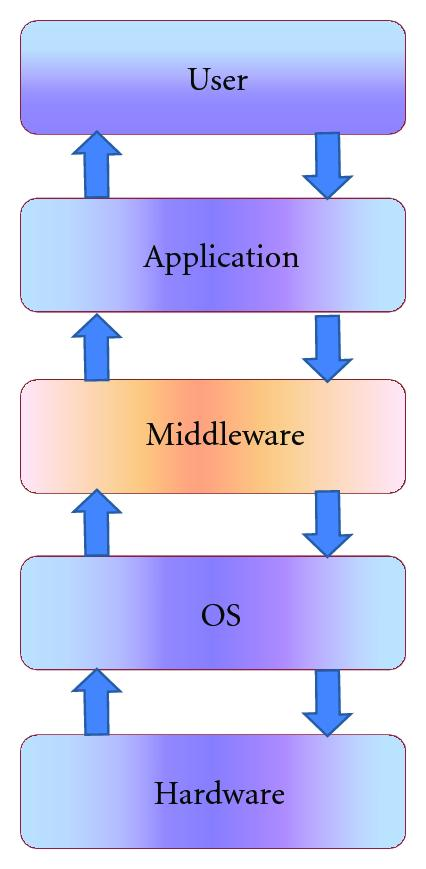
\includegraphics[width=0.3\textwidth]{figures/Introduccion/middleware.jpg}
		\caption{Estructura del funcionamiento del middleware}
		\label{fig.middleware}
		\end{center}
\end{figure}

Algunos de estos middlewares robóticos son:

\begin{itemize}
	\item \acrfull{ros} \footnote{\url{http://www.ros.org/}}: Es el software más usado en el mundo para la programación de robots. Es un entorno de programación de código abierto mantenido por la Open Source Robotics Foundation (OSRF). Ofrece una colección de herramientas, bibliotecas y convenciones que tienen como objetivo simplificar la tarea de crear un comportamiento robótico complejo y robusto en una amplia variedad de plataformas robóticas. La librería está orientada para un sistema UNIX (Ubuntu (Linux)), aunque también se está adaptando a otros sistemas operativos como Fedora, MacOS-X, Arch, Gentoo, OpenSUSE, Slackware, Debian o Microsoft Windows, considerados como ``experimentales''.
	
	\item Orca \footnote{\url{http://orca-robotics.sourceforge.net/}}: Es un entorno de programación usado para desarrollar sistemas robóticos basados en componentes. Utiliza una biblioteca de código abierto para la comunicación y la definición de interfaces. Todos sus componentes están escritos en C ++ y tiene ejemplos en Java, Python y PHP. Da soporte completo para Linux. Además, interfaces, bibliotecas principales y algunos componentes se compilan en Windows XP y hay compilaciones experimentales en MacOS-X.

	\item Player/Stage Project \footnote{\url{http://playerstage.sourceforge.net/}}: Es un proyecto que desarrolla software libre que permite la investigación de robots y sensores. Su servidor es uno de los interfaces de control de robots más utilizados del mundo, así como sus backends de simulación, Gazebo y Stage. Su modelo cliente-servidor permite que los programas de control del robot se escriban en cualquier lenguaje de programación y se ejecuten en cualquier ordenador con una conexión de red al robot. Es compatible con una amplia variedad de robots y accesorios móviles como el robot Kinect de Microsoft o la aspiradora Roomba de iRobot. Player Project funciona en Linux, Solaris, * BSD y Mac OSX (Darwin).

	\item RT-middleware \footnote{\url{http://www.openrtm.org}}: Tiene como objetivo establecer una plataforma basada en la tecnología de objetos distribuidos. RT-middleware soporta la construcción de varios sistemas robotizados en red mediante la integración de varios elementos robóticos habilitados para dicha red, denominados RT-Components. Los sistemas robóticos a los a los que da soporte no son necesariamente robots de un solo cuerpo, como robots móviles o robots humanoides, sino más generalmente ``cualquier sistema de red inteligente que utilice tecnología robótica y que pueda realizar tareas en el mundo real''. Por ejemplo, esto también incluye sistemas que aunque no se parecen a los robots utilizan tecnología robótica, como un soporte de vida diaria o sistemas de enfermería en los que varios sensores y actuadores colaboran a través de una tecnología de redes. Da soporte para Linux y Windows y tiene versiones en C++, Java y Python.

	\item JdeRobot \footnote{\url{http://jderobot.org}}: Es un entorno de programación utilizado para desarrollar aplicaciones en robótica y visión por computadora. Ha sido diseñado para ayudar en la programación de software inteligente. Principalmente, está escrito en C++ y proporciona un entorno de programación basado en componentes distribuido en el que el programa de aplicación está compuesto por una colección de varios componentes asincrónicos concurrentes. Los componentes pueden ejecutarse en diferentes equipos y están conectados mediante el middleware de comunicaciones ICE (Internet Communications Engine). Los componentes pueden escribirse en C++, Python o Java y todos ellos interactúan a través de interfaces ICE.

\end{itemize}

\subsection{Bibliotecas}
En informática, una biblioteca es un conjunto de implementaciones funcionales, codificadas en un lenguaje de programación, que ofrece una interfaz bien definida para la funcionalidad que se invoca. Su fin es ser utilizada por otros programas, independientes y de forma simultánea. Las bibliotecas pueden vincularse a un programa (o a otra biblioteca) en distintos puntos del desarrollo o la ejecución de dicho programa. Algunas de las bibliotecas utilizadas en robótica son:

\begin{itemize}
	\item OpenCV \footnote{\url{http://opencv.org/}}: Es una biblioteca libre de visión artificial originalmente desarrollada por Intel. Contiene más de quinientas funciones que abarcan una gran gama de áreas en el proceso de visión, como reconocimiento de objetos, reconocimiento facial, calibración de cámaras, visión estéreo y visión robótica. Originalmente, OpenCV fue escrita en C++. Actualmente, la librería dispone de interfaces en C++, C, Python, Java y MATLAB. Es multiplataforma, existiendo versiones para GNU/Linux, Mac OSX, Windows y Android.
	
	\item PLC \footnote{\url{http://pointclouds.org/}}: Se utiliza para el procesamiento digital de imágenes mediante el tratamiento de nubes de puntos aleatorios. Contiene numerosos algoritmos de última generación que incluyen filtrado, estimación de características, reconstrucción de superficies, ajuste de modelos y segmentación entre otros. Para simplificar el desarrollo, PCL se divide en una serie de bibliotecas de código más pequeñas, que se pueden compilar por separado. Es multiplataforma y ha sido compilado con éxito en Linux, Mac OSX, Windows y Android / iOS . 
\end{itemize}

\subsection{Simuladores}
Los simuladores son muy utilizados en robótica debido a que, normalmente, los robots suelen ser muy costosos. Mediante el uso de estos simuladores se consigue poder hacer todo tipo de pruebas con los robots sin ningún riesgo de dañar o romper el equipo. Estos simuladores representan de manera muy realista el entorno y los robots, por lo que es muy recomendable usarlos antes de probar los programas o aplicaciones creados en robots reales. Algunos de los simuladores más utilizados son:

\begin{itemize}
	\item Gazebo \footnote{\url{http://gazebosim.org/}}: Permite probar rápidamente algoritmos, diseñar robots, realizar pruebas de regresión y entrenar sistemas de inteligencia artificial utilizando escenarios realistas.  Ofrece la capacidad de simular de forma precisa y eficiente poblaciones de robots en complejos ambientes tanto interiores como exteriores. Posee un robusto motor de física, gráficos de alta calidad y cómodas interfaces gráficas. Da soporte a en Linux, Solaris, * BSD y Mac OSX (Darwin).
	
	\item Stage \footnote{\url{http://playerstage.sourceforge.net/doc/stage-svn/}}: Simula una población de robots móviles, sensores y objetos en un entorno bidimensional de mapas de bits. Está diseñado para soportar la investigación en sistemas autónomos multi-agentes, por lo que proporciona modelos relativamente simples y computacionalmente baratos de muchos dispositivos en lugar de intentar emular dispositivos con gran fidelidad. Normalmente utiliza plugins del módulo de Player y librerías escritas en C++. Funciona en los sistemas operativos en Linux, Solaris, * BSD y Mac OSX (Darwin).
\end{itemize}


\section{Robótica en docencia}
La robótica educativa es un medio de aprendizaje, en el cual participan personas con motivación por el diseño y la construcción de creaciones propias. Esta disciplina se puede enseñar a estudiantes con muy diferentes niveles educativos. \\

La robótica educativa ha crecido muy rápidamente en la última década y está en continuo desarrollo. Los robots están incorporándose en nuestra vida cotidiana, pasando de la industria a los hogares. Pero el propósito de utilizar la robótica en la educación, a diferentes niveles de enseñanza, va más allá de adquirir conocimiento en el campo de la robótica. Lo que se pretende es que el alumno sea capaz de aprender temas multidisciplinarios (electrónica, informática, mecánica, física, etc), comprenda conceptos abstractos y complejos de ciencia y tecnología, y adquiriera competencias básicas que son necesarias en la sociedad de hoy día; como son: el aprendizaje colaborativo y la toma de decisión en equipo, entre otras. Normalmente, la metodología utilizada para impartir cursos de robótica es \acrfull{stem}. \\

La robótica en la docencia intenta despertar el interés de los estudiantes transformando las asignaturas tradicionales en más atractivas e integradoras, ya que crea entornos de aprendizaje propicios que recrean los problemas del entorno que los rodea. \\

\subsection{Robótica en primaria y secundaria}

En los centros de enseñanza primaria y secundaria se imparte la robótica con frecuencia, mediante plataformas como los robots LEGO Mindstorms o placas Arduino. Se suelen enseñar conceptos básicos de sensores y actuadores empleando lenguajes gráficos como Scratch y Blockly. \\

\textbf{Plataformas hardware:} 
\begin{itemize}
	\item Arduino: Es una compañía de hardware libre y una comunidad tecnológica que diseña y manufactura placas de desarrollo de hardware, compuestas por microcontroladores, elementos pasivos y activos. Por otro lado, las placas son programadas a través de un entorno de desarrollo, el cual compila el código al modelo seleccionado de placa. El hardware consiste en una placa de circuito impreso con un microcontrolador, usualmente Atmel AVR, puertos digitales y analógicos de entrada/salida,  los cuales pueden conectarse a placas de expansión (shields), que amplían los funcionamientos de la placa Arduino. Asimismo, posee un puerto de conexión USB desde donde se puede alimentar la placa y establecer comunicación con el ordenador.
	
	\begin{figure}[H]
  	  \begin{center}
    	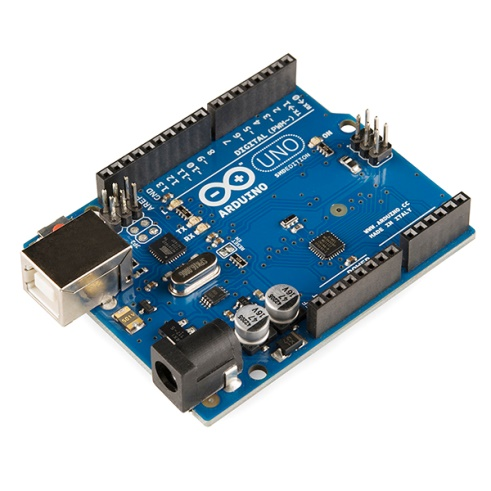
\includegraphics[width=0.3\textwidth]{figures/Introduccion/arduino.jpg}
			\caption{Placa Arduino}
			\label{fig.arduino}
	  		\end{center}
	\end{figure}
	
	\item Mbot: es un kit de robótica para que los niños se inicien en la robótica, programación y electrónica. Utiliza un  entorno de programación gráfica basada en Scratch 2.0
y es compatible con Arduino. Los niños pueden programar fácilmente el mBot sin escribir códigos y usar lenguajes de programación difíciles. Los usuarios también pueden usar la aplicación Makeblock para controlar sus robots.
	\begin{figure}[H]
  	  \begin{center}
    	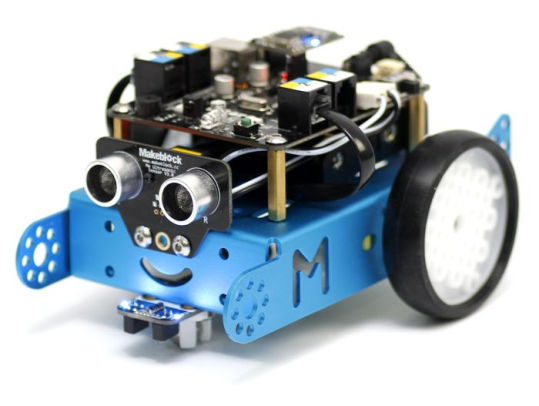
\includegraphics[width=0.3\textwidth]{figures/Introduccion/mbot.jpg}
			\caption{Robot mBot v1.1}
			\label{fig.mbot}
	  		\end{center}
	\end{figure}
\end{itemize}

\textbf{Plataformas software:} 
\begin{itemize}
	\item Scratch: Es un lenguaje de programación visual desarrollado por el MIT Media Lab. Desde 2013, Scratch 2 está disponible en línea y como aplicación de escritorio para Windows, OS X y Linux (requiere Adobe Air). Se empezó a usar Scratch como lenguaje introductorio por su relativa facilidad para desarrollar programas y  porque las habilidades adquiridas mediante Scratch se pueden aplicar a otros lenguajes básicos de programación como Python y Java. El uso de Scratch permite a las personas jóvenes a entender la lógica básica de la programación dirigida por eventos con múltiples objetos activos llamados sprites (llamados "objetos" en la versión en castellano de Scratch). Los sprites pueden pintarse como gráficos vectoriales o mapa de bits, desde la propia web de Scratch usando un simple editor que es parte del proyecto, o pueden también importarse desde fuentes externas incluyendo webcams.
	\item Lenguaje Arduino: Para decirle a la placa de Arduino qué hacer se utiliza el lenguaje de programación Arduino y su entorno de desarrollo. El software de código abierto Arduino (IDE) hace que sea fácil escribir código. Se ejecuta en Windows, Mac OS X y Linux. El entorno está escrito en Java y está basado en Processing. 
Este software se puede usar con cualquier placa Arduino.
\end{itemize}

Como entorno educativo, JdeRobot ha desarrollado JdeRobot-Kids. El objetivo principal del curso es enseñar conceptos básicos de tecnología a los alumnos e iniciarles en robótica y programación. También introduce de manera atractiva conceptos interesantes de mecánica, electrónica e informática. El carácter del curso es práctico y  ayuda a estructurar el pensamiento, a organizar las acciones en pasos para resolver un problema y a fomentar el espíritu analítico. Emplean dos plataformas concretas: ArduinoRobot y un Arduino estandard montado desde piezas y como lenguaje de programación Python y Scratch. 


\subsection{Robótica en universidades}

En la docencia universitaria se imparten clases de robótica en los Grados y los Postgrados, en concreto en escuelas de ingeniería. En España, se puede ver la robótica integrada en el ``Grado en Ingeniería Robótica'' de la Universidad de Alicante, y los Grados de ``Electrónica industrial y automática'' o en ``Ingeniería Electrónica, Robótica y Mecatrónica'' en diversas universidades. \\

En los estudios de Postgrado existen Másteres destacados como el ``Máster de Visión Artificial'' en diferentes universidades. \\

En el ámbito internacional se pueden destacar universidades especializadas en robótica como el MIT, Stanford, Georgia Institute of Technology, etc. \\

Cabe destacar el entorno de enseñanza robótica TheConstructSim \footnote{\url{http://www.theconstructsim.com/}} cuyo objetivo es enseñar a programar ROS.  Contiene una serie de tutoriales ROS en línea vinculados a simulaciones en línea, que brindan las herramientas y el conocimiento necesario para comprender y crear cualquier desarrollo de robótica basado en ROS. Usa robots reales simulados y solo se necesita un navegador web por lo que no requiere instalación.


\section{JdeRobot-Academy}
La Universidad Rey Juan Carlos cuenta con la plataforma de robótica JdeRobot, que posee un entorno académico conocido como JdeRobot-Academy. Este entorno educativo se ha empleado con éxito en diferentes asignaturas, como son ``Visión en Robótica'' del Máster de Visión Artificial, o ``Robótica'' del Grado de Ingeniería Telemática. Asimismo, la Universidad ofrece cursos de introducción a la robótica y a los drones, empleando dicha plataforma. \\

Está diseñado para que las prácticas, desarrolladas por los alumnos, se ejecuten en robots reales y también en simulados sin modificar el código fuente. El lenguaje de programación que se utiliza prácticas es Python debido a su sencillez y la potencia que ofrece. Para probar dichas prácticas en robots, se usa el simulador Gazebo. Este simulador permite aprender robótica aunque no se tengan los robots reales ya que dispone de una gran variedad de robots, como pueden ser drones, coches, aspiradoras o brazos mecánicos, entre otros, pudiendo abarcar distintos aspectos de la robótica. \\

Cada práctica consta de una aplicación académica, que resuelve tareas como la interfaz gráfica (GUI) o la conexión con sensores y actuadores concretos, y que queda oculta para el alumno. También contiene el código del estudiante, que simplemente rellena un sencillo fichero plantilla, llamado MyAlgorithm.py, con la lógica del robot, logrando así que se centre solamente en la creación y desarrollo de los algoritmos de percepción, planificación y control, habituales en los robots, necesarios para la resolución de la práctica. \\

\begin{figure}[H]
  \begin{center}
    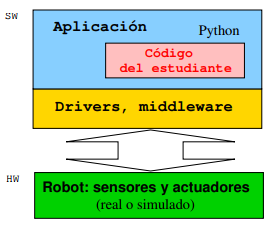
\includegraphics[width=0.3\textwidth]{figures/Introduccion/esquema.png}
		\caption{Diseño de una práctica robótica}
		\label{fig.esquema}
		\end{center}
\end{figure}

En la Figura~\ref{fig.esquema} se puede apreciar cómo está diseñada una práctica en el entorno de JdeRobot-Academy. En la capa inferior se encuentra el robot con sus actuadores (ruedas, motores...) y sensores (láseres, cámaras…) y puede ser tanto simulado como real.  En la capa intermedia se tienen los drivers y middlewares necesarios para la comunicación entre la aplicación y el robot. Y por último, en la capa superior, está la aplicación donde se analizan los datos captados por los sensores y se desarrolla el código del estudiante, tomando decisiones de actuación y planificación. \\

En la siguiente figura se puede ver la estructura que tiene cada una de las prácticas y como estan relacionados los distintos componentes.

\begin{figure}[H]
  \begin{center}
    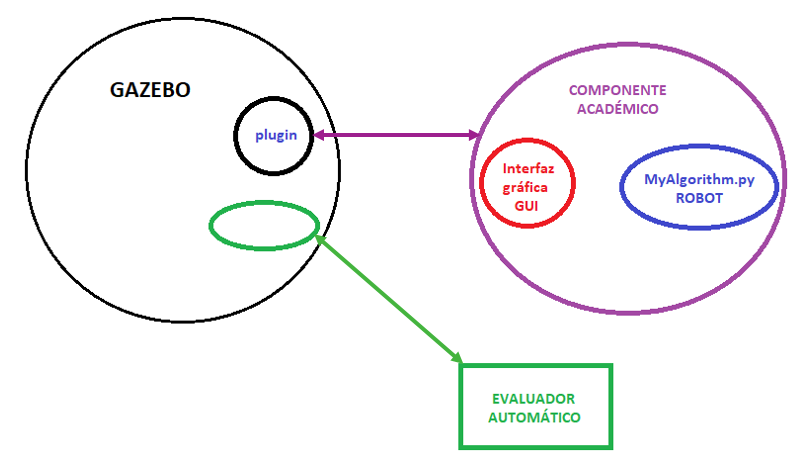
\includegraphics[width=0.5\textwidth]{figures/Introduccion/estructura.png}
		\caption{Estructura de una práctica robótica}
		\label{fig.estructura}
		\end{center}
\end{figure}


Los ámbitos principales en los que actualmente se han desarrollado prácticas son:
\begin{itemize}
	\item Visión: Aquí se pueden encontrar las prácticas ‘Color filter’, cuyo principal objetivo es el uso de filtros de color, y ‘Visual 3D reconstruction from a stereo pair of RGB cameras’ en la que se reconstruye una imagen en 3D a partir de dos cámaras de vídeo.
	\begin{figure}[H]
  	\begin{center}
    	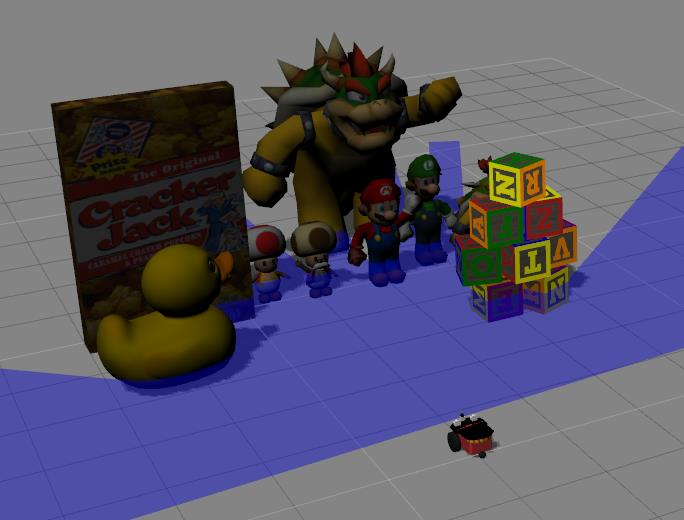
\includegraphics[width=0.4\textwidth]{figures/Introduccion/vision.jpg}
			\caption{Práctica ``Visual 3D reconstruction''}
			\label{fig.vision}
			\end{center}
	\end{figure}

	\item Coches autónomos: En este ámbito se han desarrollado las prácticas ``Visual follow-line behavior on a Formula 1'' en la cual los alumnos tienen que conseguir que un coche de Fórmula 1 logre seguir una línea roja pintada en un circuito de carreras; ``Local navigation of a Formula 1 with VFF'', su objetivo es que el alumno programe un algoritmo que consiga que un coche Fórmula 1 recorra un circuito evitando chocar con obstáculos (que son otros coches estacionados a lo largo del circuito); y ``Global navigation of a TeleTaxi with GPP'', en la cual el alumno debe programar un algoritmo para que un taxi consiga llegar a un punto del mundo en el que se encuentra clicando en una parte del mapa de dicho mundo.
	\begin{figure}[H]
  	\begin{center}
    	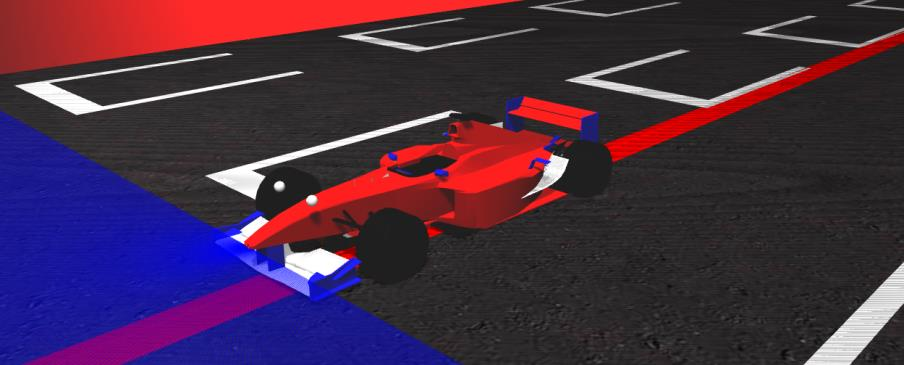
\includegraphics[width=0.4\textwidth]{figures/Introduccion/f1.jpg}
			\caption{Coche de Fórmula 1}
			\label{fig.f1}
			\end{center}
	\end{figure}

	\item Robots móviles: La práctica realizada es  ``Bump and go'', que consiste en programar la técnica ``choca-gira''  con un robot Kobuki.

	\item Drones: Es el ámbito que posee más prácticas desarrolladas. ``Drone position control navigation'' se basa en el uso de controladores PID; ``Follow the ground robot'', cuyo objetivo es conseguir que un dron siga a un robot Kobuki; ``Follow the road'', en la cual, un dron sigue una carretera; ``Drone cat and mouse'' que consiste en que un dron juega el papel de gato y tiene que atrapar al dron que tiene el papel de ratón; ``Landing on a moving car'', en esta práctica hay que lograr que un dron aterrice sobre un coche en movimiento; ``Escaping from a labyrinth using visual clue'', el objetivo es conseguir que un dron salga de un laberinto siguiendo las flechas ubicadas a lo largo de dicho laberinto; y ``People rescue after an earthquake'' que consiste en que un dron detecte personas y marque la posición en la que se encuentran.
\begin{figure}[H]
  	\begin{center}
    	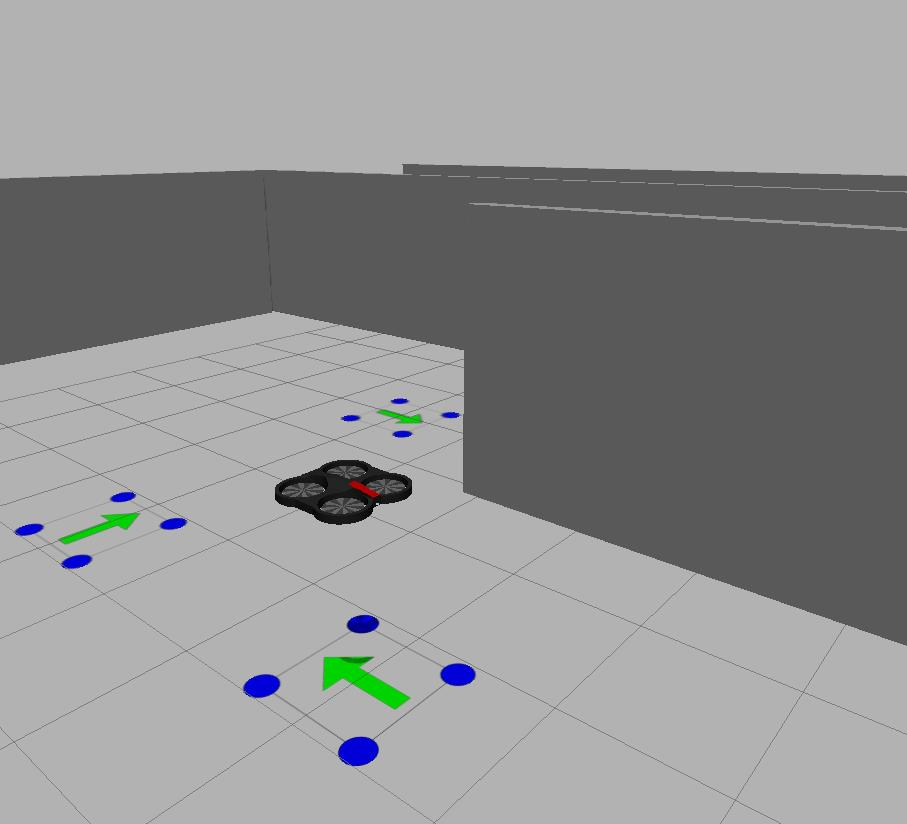
\includegraphics[width=0.4\textwidth]{figures/Introduccion/dron.jpg}
			\caption{Dron situado en un laberinto}
			\label{fig.dron}
			\end{center}
	\end{figure}
\end{itemize}

\lhead[]{CAPÍTULO \thechapter. OBJETIVOS}
\chapter{Objetivos y metodología}\label{cap.objetivos}
En este capítulo se expondrá de manera detallada el objetivo principal de este proyecto así como la metodología utilizada para su desarrollo. También se incluirá un plan de trabajo donde se explican las diferentes etapas seguidas para la realización del proyecto.

\section{Objetivos}

El objetivo principal de este trabajo es llevar a cabo dos nuevas prácticas para la plataforma JdeRobot-Academy de manera que se consiga que los alumnos que las realicen solo tengan que concentrarse en la parte de programación de robots. Además, gracias a la realización de estas prácticas el alumno adquirirá tanto conocimientos sobre programación de Python en robótica como conocimientos relacionados con el tratamiento digital de la imagen y la toma de decisiones. \\

El objetivo de la práctica ``Reconocimiento de la señal stop'' es conseguir que un coche autónomo sea capaz de reconocer una señal de stop situada a lo largo de una carretera, gracias a la cámara que lleva situada en el capó, y después, frene. Además, tiene que ser capaz de reconocer si se acercan otros coches y en caso negativo volver a arrancar. Y por último, tiene que hacer un giro a la izquierda o a la derecha de manera aleatoria. \\

En la práctica ``Aspiradora autónoma con autolocalización'', el objetivo es lograr que un robot aspirador sea capaz de barrer la mayor superficie posible de un apartamento en un tiempo limitado. Para ello, el alumno tiene que hacer uso de la capacidad de autolocalización de la aspiradora y del mapa de la casa.

\section{Metodología}
Como parte principal de la metodología se han ido acordando reuniones semanales con el tutor y los miembros del grupo de trabajo. En estas reuniones, el tutor iba revisando el trabajo realizado y marcando nuevos objetivos para la semana siguiente. Además, servían para corregir fallos y comentar las dudas que iban surgiendo a lo largo de los meses de trabajo. Gracias a esto, se podía avanzar de manera más fluida en la realización del proyecto. \\

También se ha desarrollado una bitácora en la Wiki de JdeRobot donde cada semana se redactaban los avances realizados y se añadían vídeos para mostrar los resultados obtenidos. \\

Conjuntamente a estas herramientas se ha utilizado un repositorio de Git Hub. En este repositorio se encuentra el código empleado en las prácticas, tanto el código de la infraestructura como el de las soluciones.
El desarrollo de trabajo que se ha seguido es el modelo de desarrollo en espiral. Este modelo consiste en una serie de ciclos o iteraciones que se repiten en forma de espiral como se muestra en la Figura~\ref{fig.espiral}.

\begin{figure}[H]
  \begin{center}
    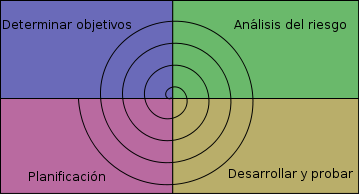
\includegraphics[width=0.6\textwidth]{figures/Objetivos/espiral.png}
		\caption{Metodología en espiral}
		\label{fig.espiral}
		\end{center}
\end{figure}

Cada ciclo consta de cuatro fases que son las siguientes:
\begin{itemize}
	\item Determinar objetivos: en esta fase se definen los objetivos que se deben de llevar a cabo para que una vez completados se pueda dar por finalizado el ciclo.

	\item Análisis del riesgo: en la segunda fase se evalúa que problemas es posible encontrarse al empezar el desarrollo.

	\item Desarrollar y probar: en la tercera fase, una vez evaluados los riesgos se procede al propio desarrollo del trabajo realizando distintas pruebas para conseguir el mejor resultado.

	\item Planificación: en esta última fase se valoran los resultados obtenidos y se planifican los siguientes etapas del proyecto.
\end{itemize}

No existe un número fijo de iteraciones, deben de llevarse a cabo tantas como sean necesarias hasta completar el trabajo. \\

La adaptabilidad en el diseño del modelo de espiral en la ingeniería de software se adapta a cualquier número de cambios, que pueden ocurrir durante cualquier fase del proyecto, permitiendo minimizar los riesgos y realizar un buen desarrollo del trabajo.

\section{Plan de trabajo}

Para lograr los objetivos ya descritos, se han seguido las siguientes etapas:
\begin{itemize}
	\item Familiarización del entorno JdeRobot, mediante la descarga e instalación del software de JdeRobot además de las distintas dependencias necesarias para el correcto uso de JdeRobot. En esta etapa también se llevó a cabo la resolución de algunas prácticas anteriores de JdeRobot-Academy relacionadas con las prácticas a desarrollar.

	\item Familiarización del simulador Gazebo. En esta etapa se han estudiado distintos ejemplos disponibles en la web de Gazebo y de JdeRobot. Además, se han comprendido los distintos plugins necesarios para el desarrollo del trabajo lo que implicó un aprendizaje básico del lenguaje de programación C++.

	\item Crear los mundos y plugins necesarios de Gazebo.  Se modificaron distintos plugins ya creados para adaptarlos a las prácticas que se iban a desarrollar. También se diseñaron los mundos que se han utilizado en cada ejercicio incluyendo en dichos mundos tanto los modelos de objetos y obstáculos como los de los robots y coches.

	\item Desarrollar la infraestructura, que consistirá principalmente en crear la interfaz gráfica, utilizando la herramienta PyQt5, para que el alumno pueda resolver las prácticas de manera más sencilla e intuitiva.

	\item Desarrollar un evaluador automático, para que el alumno sepa de manera automática que nota ha obtenido con el código que programe. Este evaluador medirá distintos parámetros y calculará una nota final. También ha sido necesario el uso de la herramienta PyQt5.

	\item Realizar las soluciones. En esta etapa se ha realizado un algoritmo por cada práctica.

	\item Redactar los enunciados, donde se explica el contenido de cada práctica.
\end{itemize}


\lhead[]{CAPÍTULO \thechapter. INFRAESTRUCTURA}
\chapter{Infraestructura}\label{cap.infraestructura}
En este capítulo se explicarán los principales ingredientes software en los que nos hemos apoyado para desarrollar el trabajo. Tales como el simulador Gazebo (con el cual se pueden simular robots con sus sensores y actuadores), el entorno JdeRobot, la biblioteca de OpenCV (empleada en todo lo relacionado con el tratamiento de imagen), PyQt (para el desarrollo de la interfaz gráfica) y Python como lenguaje de programación.

\section{Simulador Gazebo}

Como se argumentó en el Capítulo 1, el simulador Gazebo es uno de los ejes principales de JdeRobot-Academy. Es un simulador usado en robótica que permite realizar diversos escenarios tridimensionales donde probar nuestro software. A la hora de desarrollar el software es necesario hacer pruebas, las cuales saldrían muy costosas si se probaran en robots reales (podría no funcionar correctamente y que el robot se rompiera). Por esta razón es muy útil el empleo de simuladores, pues se pueden realizar las pruebas que se quieran sin peligro de que el robot se estropee. Con los simuladores se pueden diseñar robots y escenarios realistas donde ejecutar los algoritmos creados.

\begin{figure}[H]
  \begin{center}
    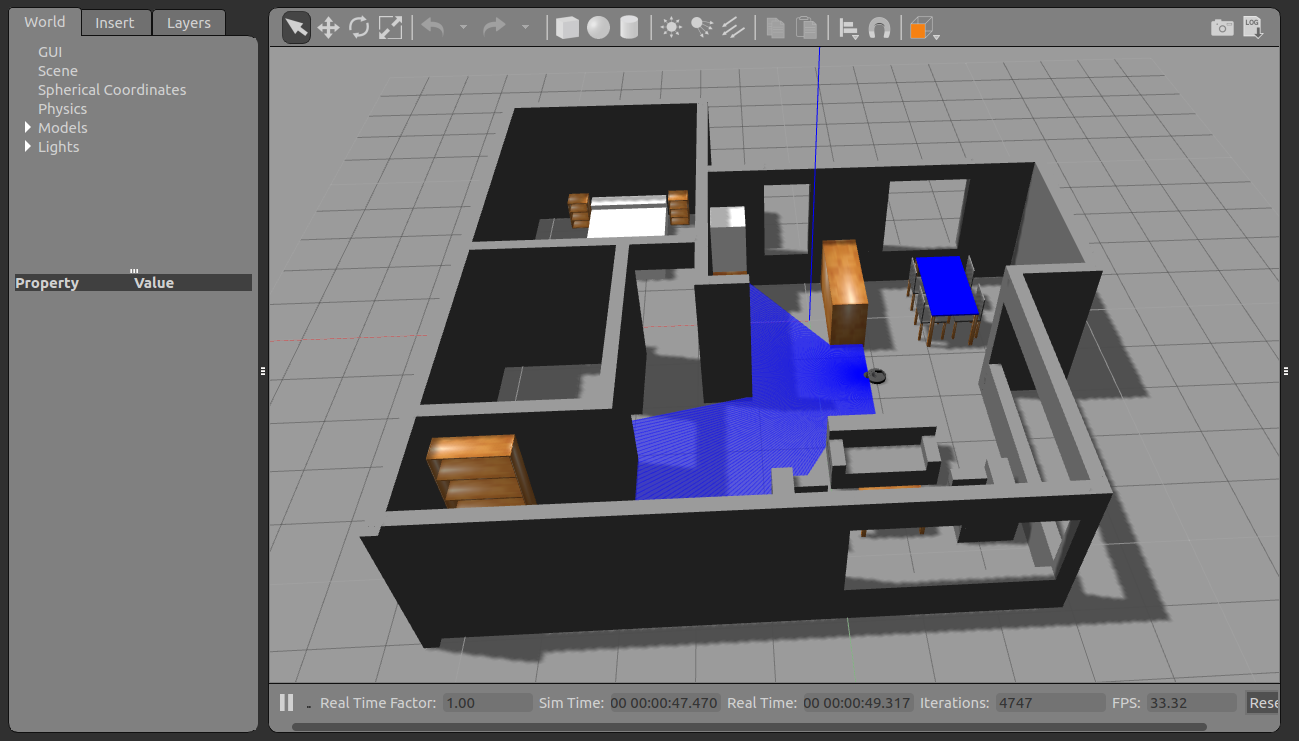
\includegraphics[width=0.8\textwidth]{figures/Infraestructura/gazebo.png}
		\caption{Simulador Gazebo}
		\label{fig.gazebo}
		\end{center}
\end{figure}

 
Gazebo es un programa de código abierto distribuido bajo licencia de Apache 2.0. Se emplea en el desarrollo de aplicaciones robóticas y en inteligencia artificial. Es capaz de simular robots, objetos y sensores en entornos complejos de interior y exterior. Tiene gráficos de gran calidad y un robusto motor de física (masa del robot, rozamiento, inercia, amortiguamiento, etc.). En la Figura~\ref{fig.gazebo} aparece el mundo utilizado en la práctica de ``Aspiradora autónoma con autolocalización''. Se puede apreciar como Gazebo simula tanto objetos (camas, sofás, muebles...) como robots, en este caso, un robot aspirador. \\

Fue elegido para realizar el DARPA Robotics Challenge (2012-2015) y está mantenido por la Fundación Robótica de Código Abierto (OSRF). \\

En este proyecto se emplea la versión 7 de Gazebo, la cual se usará para crear los diferentes entornos y para probar nuestros algoritmos.  Gracias a Gazebo se pueden incluir texturas, luces y sombras en los escenarios, así como simular física como por ejemplo choques, empujes, gravedad, etc. Además, incluye diversos sensores, como pueden ser cámaras y lásers, los cuales podrán ser incorporados en los robots que empleemos. Todo ello hace que sea una herramienta muy potente y de gran ayuda en el mundo de la robótica.\\

Los mundos simulados con Gazebo son 3D, que se cargan a partir de ficheros con extensión ``.world''. Son ficheros definidos en \acrfull{sdf} que es un formato \acrfull{xml} que describe objetos y entornos para simuladores, visualización y control de robots. Originalmente fue desarrollado como parte del simulador Gazebo pero con los años se ha convertido en un formato estable, robusto y extensible capaz de describir todos los aspectos de los robots, los objetos estáticos y dinámicos, la iluminación, el terreno e incluso la física.\\

Se puede describir con precisión todos los aspectos de un robot que usa SDF, ya sea un robot que sea un simple chasis con ruedas o un humanoide. Además de los atributos cinemáticos y dinámicos, se pueden definir sensores, propiedades de superficie, texturas, fricción de la junta y muchas más propiedades para un robot. Estas características permiten usar SDF para simulación, visualización, planificación de movimiento y control de robot. Los modelos de robots que se emplean en la simulación pueden ser creados mediante algún programa de modelado 3D como Blender o Sketchup. Estos robots simulados necesitan ser dotados de inteligencia para lo cual se emplean plugins. Éstos, pueden dotar al robot de inteligencia u ofrecer la información de sus sensores a aplicaciones externas y recibir de éstas comandos para los actuadores de los robots.


\section{Entorno JdeRobot}

\section{Lenguaje de programación Python}

\section{Biblioteca OpenCV}

\section{PyQt}
\lhead[]{CAPÍTULO \thechapter. STOP}
\chapter{Práctica: Reconocimiento de la señal Stop}\label{cap.stop}
En este capítulo se expondrá la creación de una nueva práctica para la plataforma de JdeRobot-Academy, llamada ``Reconocimiento de la señal stop''. Se explicará el desarrollo de su infraestructura, su componente académico correspondiente, así como la solución de referencia llevada a cabo. 

\section{Enunciado} \label{sec.enunciado}
El objetivo principal de esta práctica es conseguir que un coche autónomo sea capaz de reconocer una señal de stop. Además, deberá frenar a tiempo en un cruce y después, si no detecta coches, volver a arrancar y realizar un giro a la izquierda o a la derecha de manera aleatoria. El modelo del coche utilizado está dotado de cámaras de vídeo para visualizar el entorno, un sensor de posición y actuadores de movimiento que permiten controlar tanto la velocidad lineal como la de giro. \\

En esta práctica el alumno tiene que programar un algoritmo que cumpla todos los objetivos descritos, evitando que el coche autónomo choque con otros coches u obstáculos de su entorno. En la interfaz gráfica del componente académico se pueden visualizar las imágenes captadas por las cámaras.\\

El algoritmo responde a un control reactivo, por lo que en cada instante actuará en función de los datos captados por los sensores permitiendo controlar el movimiento del coche y reaccionar a distintos imprevistos.

\section{Infraestructura}
En este apartado se describirá el entorno que se ha creado para poder realizar la práctica ``Reconocimiento de la señal stop''. Primero se describirá el modelo del coche utilizado, incluyendo sus sensores y actuadores. Después, se explicará el mundo simulado por el cual se moverá el coche. 

\subsection{Modelo coche Opel}
Para esta práctica se ha creado un nuevo modelo de coche autónomo. El robot está basado en un modelo de coche Opel. Este modelo de coche se denomina \textit{``Opel''} y se puede ver en Figura~\ref{fig.cocheOpel}. Posee tres cámaras de vídeo que se usarán para la detección de la señal de stop y la detección de otros coches; un sensor de posición, que se utilizará para obtener su orientación al realizar los giros, tanto a la izquierda como a la derecha; y motores que le permiten moverse por el mundo de Gazebo.

\begin{figure}[H]
  \begin{center}
    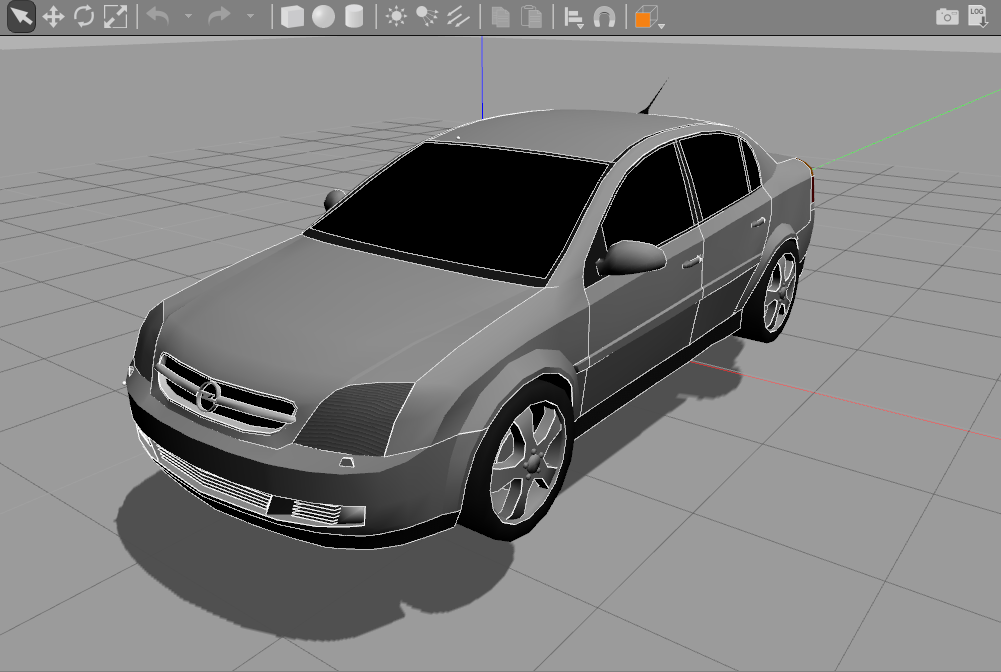
\includegraphics[width=0.7\textwidth]{figures/Stop/cocheOpel.png}
		\caption{Modelo coche Opel}
		\label{fig.cocheOpel}
  \end{center}
\end{figure}

En esta práctica se han empleado los siguientes \textit{plugins} para este modelo:

\begin{itemize}
\item	\textit{OpelMotors}: El componente académico interactúa con este \textit{plugin}. Este \textit{plugin} permite dotar al componente de velocidad, tanto velocidad de tracción como velocidad de rotación.
\item	\textit{camera\_dump}: Este \textit{plugin} será empleado por los componentes para tener visión del entorno.
\item	\textit{Pose3D}: Este \textit{plugin} se emplea para obtener la posición del coche en tiempo real y su orientación.
\end{itemize}


\subsubsection{Cámaras de vídeo}
En este coche se han instalado 3 cámaras de vídeo. Las imágenes captadas tienen un tamaño de 640 x 480 píxeles y están basadas en el modelo de color \acrshort{rgb} (cada uno de estos tres canales esta codificado con 1 byte). El rango de profundidad de visión de las cámaras abarca desde 10 centímetros hasta 35 metros. Una de las cámaras está situada en el centro del techo (ligeramente a la derecha), otra al lado del faro derecho (orientada hacia a la derecha) y la última, a lado del faro izquierdo (orientada hacia a la izquierda). De esta manera, conseguimos un campo de visión más amplio. La cámara central se usará para el proceso de detección de la señal de stop y la carretera, y las cámaras laterales, para la detección de otros coches.

\subsection{Modelo car}
Se han añadido dos coches adicionales que se mueven de manera automática a lo largo de una de las carretera para simular el tráfico de una calle. Ambos coches utilizan la misma malla visual que el modelo Opel por lo que tienen el mismo aspecto. \\

Para conseguir que los coches se muevan de manera automática, se ha creado un nuevo \textit{plugin} llamado \textit{``carplugin''}. Este \textit{plugin} dota de velocidad lineal constante al modelo en su eje x y, dependiendo de su posición en el simulador Gazebo, tomará dirección positiva o negativa.


\subsection{Modelo stop\_sign}
Debido a que el objetivo principal de la práctica es reconocer una señal de stop, se ha añadido el modelo \textit{``stop\_sign''}. Este modelo se puede ver en la Figura~\ref{fig.stopSign}.

\begin{figure}[H]
  \begin{center}
    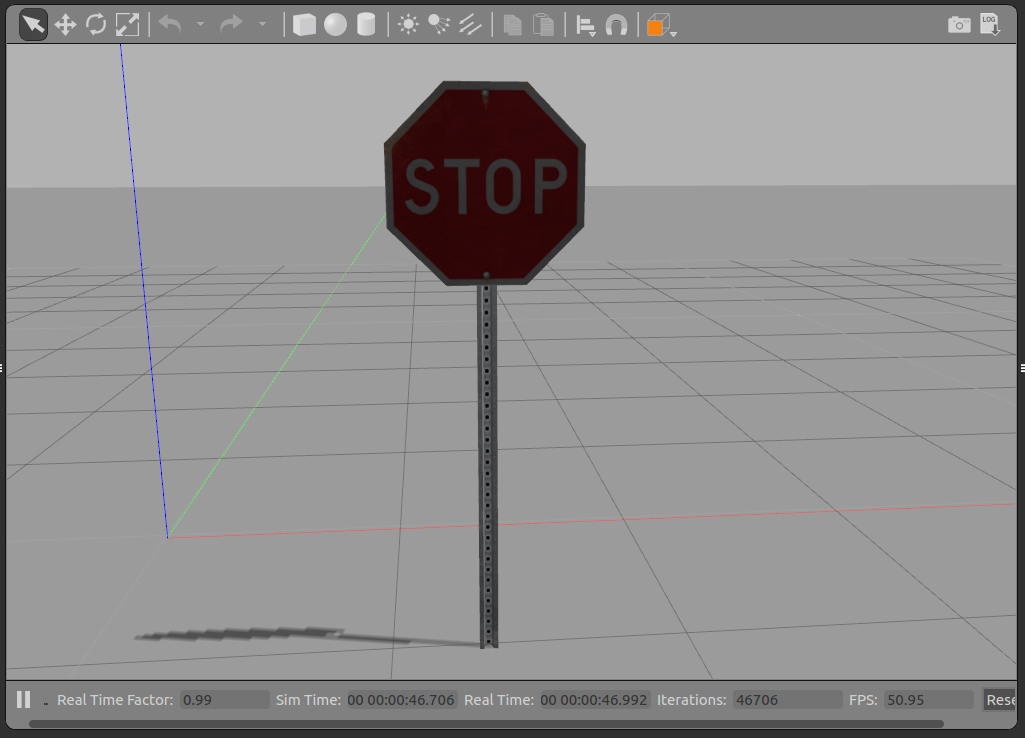
\includegraphics[width=0.5\textwidth]{figures/Stop/stopSign.png}
		\caption{Modelo stop\_sign}
		\label{fig.stopSign}
		\end{center}
\end{figure}

\subsection{Modelo StopW}
Ha sido necesario crear el modelo de un cruce de carreteras por donde circularán los coches utilizados en esta práctica. Este modelo se ha denominado \textit{``StopW''} y se puede ver en la Figura~\ref{fig.stopW}. 

\begin{figure}[H]
  \begin{center}
    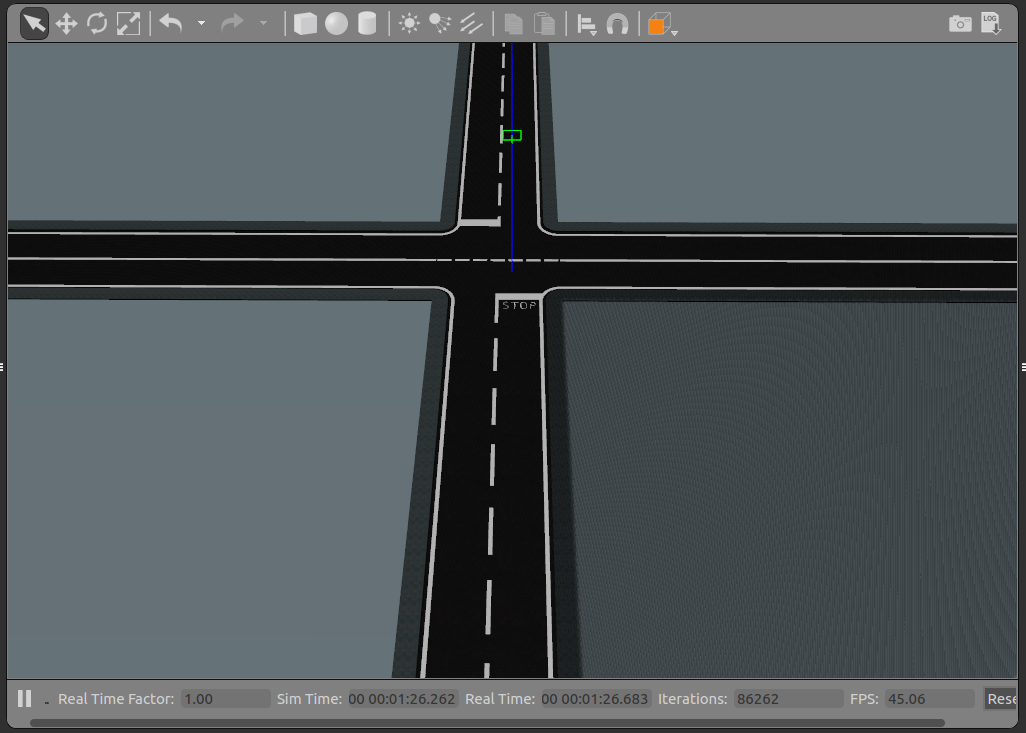
\includegraphics[width=0.8\textwidth]{figures/Stop/stopW.png}
		\caption{Modelo stopW}
		\label{fig.stopW}
		\end{center}
\end{figure}

\subsection{Mundo de Gazebo}
Los mundos que se simulan con Gazebo son mundos 3D. Estos mundos se cargan en ficheros con extensión .world, que no son más que ficheros \acrshort{xml} definidos en el lenguaje \acrshort{sdf}. Este lenguaje contiene una descripción completa de todos los elementos que tiene el mundo y los robots.\\

El mundo creado en Gazebo está formado por un modelo de cruce de carreteras \textit{``stopW''}, dos señales de stop con el modelo \textit{``stop\_sign''}, poseerá 2 coches que se mueven de manera autómatica empleando el modelo \textit{``car''} y se incluirá el modelo del coche \textit{``Opel''}, que ejecutará la solución desarrollada. Por útimo, para dotar de realismo al mundo se han añadido algunos modelos que tiene Gazebo:

\begin{itemize}
\item	Modelo \textit{sun}: Añade una fuente de luz global a la escena.
\item	Modelo \textit{house\_1}, modelo \textit{house\_2}, modelo \textit{house\_3}: Se han utilizado distintos modelos de casas.
\item	Modelo \textit{gas\_station}: Se ha añadido el modelo de una gasolinera.
\item	Modelo \textit{lamp\_post}: Se han añadido un total de 14 farolas situadas a lo largo de las carreteras.
\end{itemize}

Para tener este escenario se ha creado un mundo en Gazebo llamado \textit{``stop.world''}:

\vspace{20pt}
	\begin{lstlisting}[frame=single]
<?xml version="1.0"?>
<sdf version="1.4">
  <world name="default">
  
    <scene>
      <grid>false</grid>
    </scene>
  
    <!-- A global light source -->
    <include>
      <uri>model://sun</uri>
      <pose>1.5 -30 100 0 0 0</pose>
    </include>
    
    <!-- Stop signs -->
    <include>
      <static>true</static>
      <uri>model://gazebo/models/stop_sign</uri>
      <pose>3.5 -3.5 0 0 0 0</pose>
    </include>
    
    <include>
      <static>true</static>
      <uri>model://gazebo/models/stop_sign</uri>
      <pose>-3 3 0 0 0 3.15</pose>
    </include>
    
    
    <!-- Houses -->
    <include>
      <uri>model://house_1</uri>
      <pose>-9.5 8.5 0 0 0 0</pose>
    </include>
    
    <include>
      <uri>model://house_2</uri>
      <pose>-25 7.5 0 0 0 0</pose>
    </include>
    
    <include>
      <uri>model://house_3</uri>
      <pose>-5.5 -7 0 0 0 1.55</pose>
    </include>
    
    
    <!-- A gas station -->
    <include>
      <uri>model://gas_station</uri>
      <pose>10 14 0 0 0 1.55</pose>
    </include>
    
    
    <!-- Lamps -->
    <include>
      <uri>model://lamp_post</uri>
      <pose>-3 13 0 0 0 1.55</pose>
    </include>
    <include>
      <uri>model://lamp_post</uri>
      <pose>3 23 0 0 0 -1.55</pose>
    </include>
    <include>
      <uri>model://lamp_post</uri>
      <pose>-3 33 0 0 0 1.55</pose>
    </include>
    
    <include>
      <uri>model://lamp_post</uri>
      <pose>-3 -3 0 0 0 1.55</pose>
    </include>
    <include>
      <uri>model://lamp_post</uri>
      <pose>3 -13 0 0 0 -1.55</pose>
    </include>
    <include>
      <uri>model://lamp_post</uri>
      <pose>-3 -23 0 0 0 1.55</pose>
    </include>
    <include>
      <uri>model://lamp_post</uri>
      <pose>3 -33 0 0 0 -1.55</pose>
    </include>
    
    <include>
      <uri>model://lamp_post</uri>
      <pose>3 3 0 0 0 0</pose>
    </include>
    <include>
      <uri>model://lamp_post</uri>
      <pose>13 -3 0 0 0 3.15</pose>
    </include>
    <include>
      <uri>model://lamp_post</uri>
      <pose>23 3 0 0 0 0</pose>
    </include>
    <include>
      <uri>model://lamp_post</uri>
      <pose>33 -3 0 0 0 3.15</pose>
    </include>

    <include>
      <uri>model://lamp_post</uri>
      <pose>-13 3 0 0 0 0</pose>
    </include>
    <include>
      <uri>model://lamp_post</uri>
      <pose>-23 -3 0 0 0 3.15</pose>
    </include>
    <include>
      <uri>model://lamp_post</uri>
      <pose>-33 3 0 0 0 0</pose>
    </include>
    

    <!-- A opel car -->
    <include>
      <uri>model://opel</uri>
      <pose>1.5 -30 0 0 0 3.14</pose> 
    </include>
    
    
    <!-- Cars -->
    <include>
      <uri>model://car</uri>
      <pose>-30 -1.5 0 0 0 1.57</pose>
    </include>
    
    <include>
      <uri>model://car</uri>
      <pose>40 1.5 0 0 0 -1.57</pose>
    </include>
    
    
    <!-- Roads -->
    <include>
      <uri>model://stopW</uri>
      <pose>0 0 0 0 0 0</pose>
    </include>
    
  </world>
</sdf>
	\end{lstlisting}


En la Figura~\ref{fig.stopWorld} se puede observar el mundo creado en Gazebo.

\begin{figure}[H]
  \begin{center}
    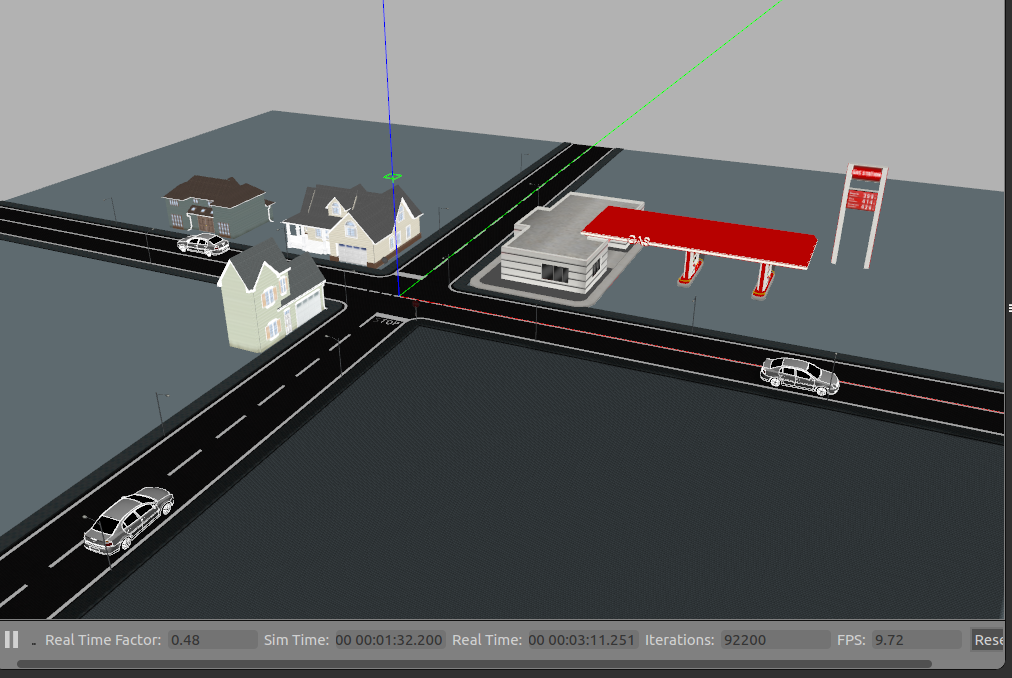
\includegraphics[width=1.0\textwidth]{figures/Stop/stopWorld.png}
		\caption{Mundo stop.world en Gazebo}
		\label{fig.stopWorld}
		\end{center}
\end{figure}


\section{Componente académico}
Se ha creado un componente académico para esta práctica que resuelve diversas funcionalidades: (a) muestra una interfaz gráfica al usuario, con distintos elementos, que permiten depurar el código de manera más sencilla; (b) ofrece acceso a sensores y actuadores en forma de métodos simples ocultando el \textit{middleware} de comunicaciones; (c) incluye código auxiliar que ayuda a programar la solución. El componente deja todo listo para que el estudiante sólo tenga que incorporar su código rellenando el método \textit{execute} en el fichero \textit{MyAlgorithm.py}.\\

Este componente ofrece al programador del algoritmo este \acrshort{api} de sensores y actuadores:

\begin{itemize}
\item 	\textit{pose3d.getX()}: Permite obtener la posición absoluta del robot en el eje X.
\item	\textit{pose3d.getY()}: Permite obtener la posición absoluta del robot en el eje Y.
\item	\textit{pose3d.getYaw()}: Permite obtener la orientación del robot con respecto al sistema de referencia de Gazebo.
\item 	\textit{motors.sendV()}: Para establecer la velocidad lineal.
\item	\textit{motors.sendW()}: Para establecer la velocidad de giro.
\item	\textit{cameraC.getImage()}: Permite obtener las imágenes captadas por la cámara situada en el techo del coche.
\item	\textit{cameraL.getImage()}: Permite obtener las imágenes captadas por la cámara situada en el faro izquierdo.
\item	\textit{cameraR.getImage()}: Permite obtener las imágenes captadas por la cámara situada en el faro derecho.
\end{itemize}

Es necesario crear un archivo de configuración (\textit{stop.cfg}) donde se indican los puertos utilizados por los distintos \textit{plugins}, la velocidad lineal máxima y la velocidad angular máxima de los motores.:

\vspace{20pt}
	\begin{lstlisting}[frame=single]
Stop.CameraC.Proxy  = cam_opel_center:default -h localhost -p 8995
Stop.CameraL.Proxy  = cam_opel_left:default -h localhost -p 8996
Stop.CameraR.Proxy  = cam_opel_right:default -h localhost -p 8997
Stop.Motors.Proxy  = Motors:default -h localhost -p 9999
Stop.Pose3D.Proxy  = Pose3D:default -h localhost -p 9989

Stop.Motors.maxV = 250
Stop.Motors.maxW = 20
	\end{lstlisting}

En esta práctica, los motores emplean el puerto 9999; el sensor de posición el puerto 9989; y las cámaras central, izquierda y derecha utilizan los puertos 8995, 8996 y 8997, respectivamente. \\

Para poder realizar todas las tareas necesarias para el funcionamiento de la práctica se emplean dos hilos de ejecución:

\begin{itemize}
\item	Hilo de control: se encarga de actualizar de manera constante los datos captados por los sensores y los datos enviados a los actuadores. Debido a que se trata de una solución reactiva es necesario que el intervalo de actualización de dichos datos sea un tiempo muy corto, en este caso, 50 ms. Si se fijara un tiempo muy grande podría ocasionar errores en la trayectoria del robot.
\item	Hilo de la \acrshort{gui}: este hilo actualiza la interfaz gráfica que se muestra al usuario. Este intervalo de actualización debe de ser también corto ya que la interfaz gráfica es una herramienta que utiliza el programador para depurar su código y debe de mostrar de manera fiable los datos del robot en tiempo real. Este intervalo también es de 50 ms.
\end{itemize}


\subsection{Interfaz gráfica}
Para que la realización de la práctica sea más fácil, se ha creado una interfaz gráfica que muestra datos importantes, relativos al robot, al usuario. Además, esta interfaz permite de manera sencilla ejecutar el código donde se desarrolla la solución correspondiente. Se ha empleado la herramienta PyQt5 para su desarrollo.\\

En la parte izquierda de la interfaz gráfica, se muestran las imágenes captadas por las tres cámaras de vídeo instaladas en el robot. Mediante estas imágenes el programador podrá verificar si está realizando correctamente el tratamiento digital de las imágenes necesario para detectar tanto la señal de stop, como la carretera o los otros coches. Las imágenes de la cámara izquierda se reproducen a la izquierda de la interfaz, las de la cámara central en el centro y las de la cámara derecha a la derecha.\\

A la derecha, hay un teleoperador que permite mover el coche manualmente. Se puede controlar tanto la velocidad lineal (en el eje vertical) como la velocidad de giro (eje horizontal). \\

En la parte inferior, aparecen dos botones. El botón situado bajo las imágenes captadas por las cámaras, permite tanto ejecutar como parar el código alojado en el archivo \textit{MyAlgorithm.py}. Con el botón que está bajo el teleoperador, se puede detener al robot si se está controlando con el teleoperador. \\

En la Figura~\ref{fig.stopGUI} se muestra el resultado de la interfaz gráfica que verá el usuario en todo momento.

\begin{figure}[H]
  \begin{center}
    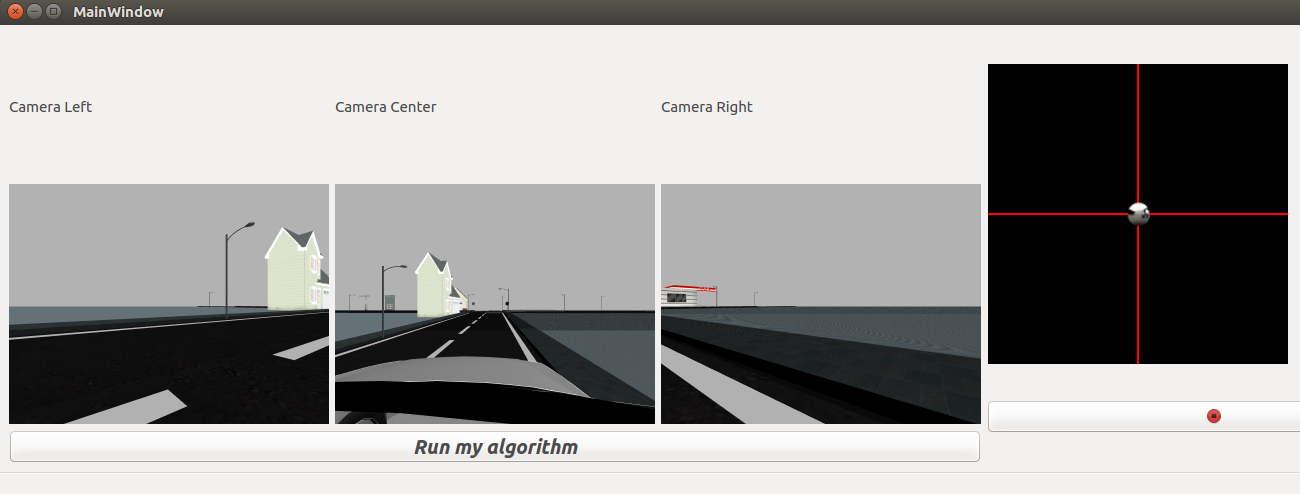
\includegraphics[width=1.0\textwidth]{figures/Stop/stopGUI.png}
		\caption{Interfaz gráfica}
		\label{fig.stopGUI}
		\end{center}
\end{figure}


\section{Solución de referencia}
La solución desarrollada para esta práctica resuelve el problema planteado de reconocer una señal de stop. La solución se ha programado en el fichero \textit{MyAlgorithm.py}, en el método \textit{``execute''}, que es el método principal de la solución. De este modo se puede crear un control reactivo, donde el coche irá tomando decisiones según los datos que vaya obteniendo de los sensores en tiempo real. Para esta práctica se ha realizado el pilotaje del robot sin una planificación de movimiento previa.\\

La solución puede dividirse en tres partes principales: (a) reconocimiento de la señal de stop y frenado del coche; (b)detección de otros coches; (c) realización del giro. 

\subsection{Reconocimiento de la señal de stop y frenado del coche}
Para detectar la señal de stop, nos basaremos en dos de sus características principales: el color y la forma. Si solo nos centráramos en el color podría llevarnos a error, ya que existen más señales viales de color rojo, por lo que necesitamos fijarnos en otra característica. En este caso nos hemos decantado por la forma ya que la señal de stop es la única señal vial que tiene forma octogonal. \\

Para llevar acabo el proceso de detección, utilizaremos las imágenes captadas por la cámara situada en el techo del coche. A estas imágenes les aplicamos un filtro de color para detectar el color rojo específico de la señal. Para ello, hemos creado la función \textit{``filterHSV''} que realizará el cambio de modelo de color de \acrshort{rgb} (Figura~\ref{fig.imgRGByHSV}) al modelo \acrshort{hsv}, el proceso de segmentación (Figura~\ref{fig.colorFilterRed}) y aplicará la operación morfológica de cierre (Figura~\ref{fig.close}) para eliminar la palabra ``STOP'' de la señal. Para fijar los valores del filtro, hemos utilizado la herramienta ``colorTuner'' de JdeRobot.\\

\begin{figure}[H]
  \begin{center}
    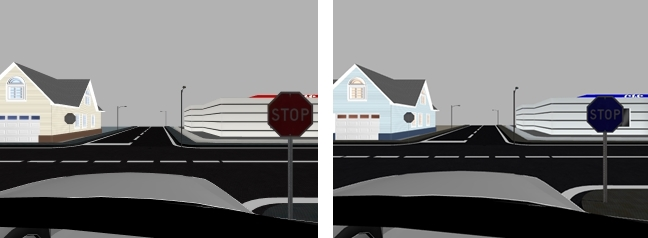
\includegraphics[width=0.8\textwidth]{figures/Stop/imgRGByHSV.jpg}
		\caption{Imagen original en RGB y en HSV}
		\label{fig.imgRGByHSV}
		\end{center}
\end{figure}

\begin{figure}[H]
  \begin{center}
    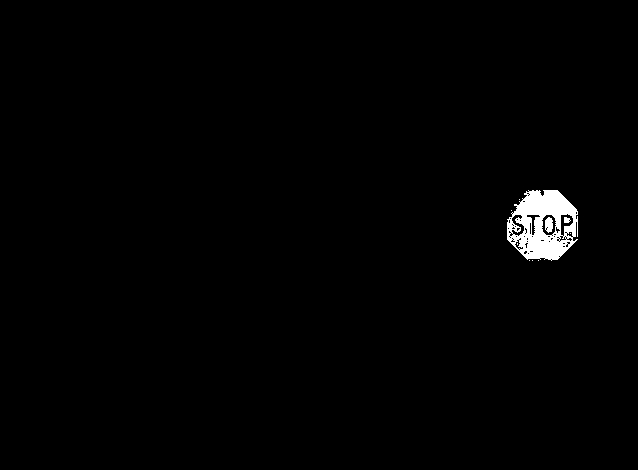
\includegraphics[width=0.5\textwidth]{figures/Stop/colorFilterRed.jpg}
		\caption{Imagen con filtro de color rojo}
		\label{fig.colorFilterRed}
		\end{center}
\end{figure}

\begin{figure}[H]
  \begin{center}
    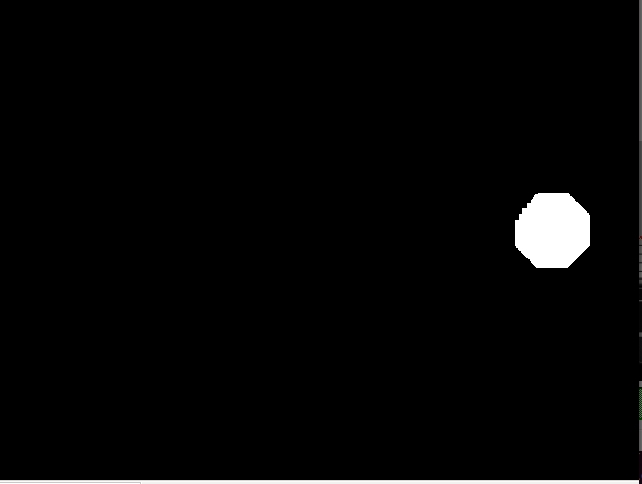
\includegraphics[width=0.5\textwidth]{figures/Stop/close.jpg}
		\caption{Imagen con cierre}
		\label{fig.close}
		\end{center}
\end{figure}


De esta manera, obtenemos una imagen binaria con la forma de la señal de stop en primer plano (blanco) (Figura~\ref{fig.close}). Esta imagen la compararemos con una plantilla de referencia para comprobar que se trata de la forma que queremos (octogonal). Para realizar esta comparación recortamos la imagen filtrada (Figura~\ref{fig.cut}) para quedarnos solo con la parte de la imagen que contiene la señal y la redimensionamos para que, tanto esta imagen como la plantilla (Figura~\ref{fig.template}), tengan el mismo tamaño y poder realizar correctamente el cotejamiento. \\

\begin{figure}[H]
  \begin{center}
    
\includegraphics[width=0.2\textwidth]{figures/Stop/cut.jpg}
		\caption{Señal de stop recortada}
		\label{fig.cut}
		\end{center}
\end{figure}

\begin{figure}[H]
  \begin{center}
    
\includegraphics[width=0.2\textwidth]{figures/Stop/template.png}
		\caption{Plantilla de referencia}
		\label{fig.template}
		\end{center}
\end{figure}

Una vez que hemos detectado la señal, el coche deberá frenar hasta situarse en el cruce de las dos carreteras. Para realizar el frenado hemos creado la función \textit{``brake''}, mediante la cual, el coche irá reduciendo su velocidad lineal según el tamaño que vaya adquiriendo la señal de stop detectada. Al principio, esta señal será pequeña ya que estará a lo lejos e irá aumentando de tamaño según el coche se vaya acercando hacia ella (Figura~\ref{fig.brake}). Para saber el tamaño de la señal, realizamos un \textit{bounding} alrededor de la señal (Figura~\ref{fig.stopRecuadro}) y, según el tamaño del recuadro, se llevarán a cabo las distintas fases del frenado, disminuyendo paulatinamente la velocidad. \\

\begin{figure}[H]
  \begin{center}
    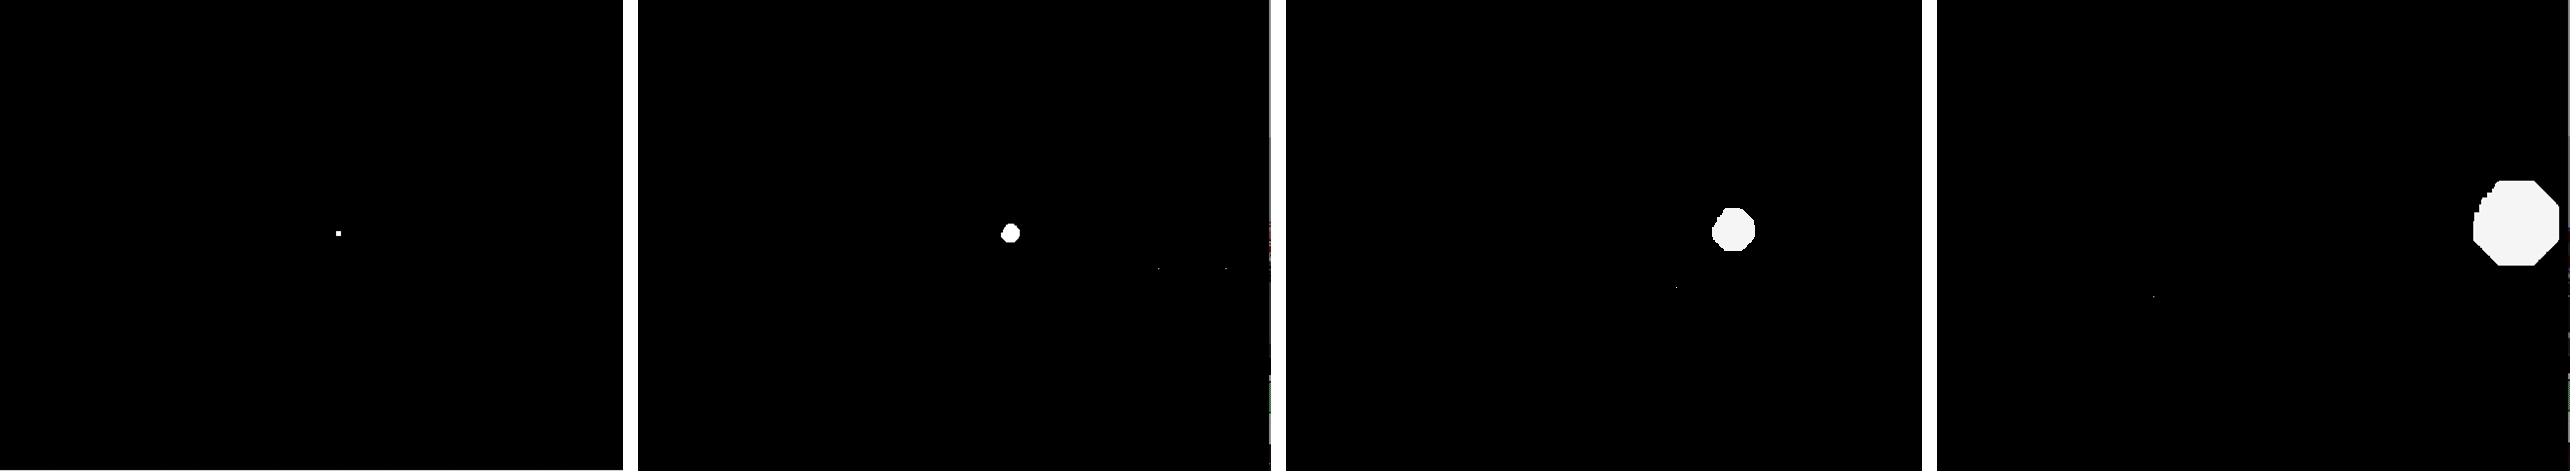
\includegraphics[width=1.0\textwidth]{figures/Stop/brake.jpg}
		\caption{Aumento del tamaño de la señal de stop}
		\label{fig.brake}
		\end{center}
\end{figure}

\begin{figure}[H]
  \begin{center}
    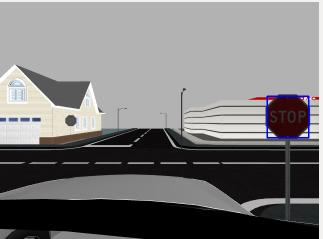
\includegraphics[width=0.5\textwidth]{figures/Stop/stopRecuadro.jpg}
		\caption{Señal de stop recuadrada}
		\label{fig.stopRecuadro}
		\end{center}
\end{figure}

\subsection{Detección de otros coches}
Después de frenar, el coche deberá saber si vienen o no otros vehículos y luego reanudar su camino. Para distinguir a los otros coches que circulan por la carretera perpendicular, nos basamos en la resta de imágenes para detectar su movimiento (ya que en este escenario serán los únicos elementos que se moverán). Usaremos las imágenes captadas por las cámaras situadas en los faros de los coches (tanto la izquierda como la derecha), las transformaremos a escala de grises y les aplicaremos un suavizado mediante un filtro de Gauss para que la detección de movimiento sea más sencilla (Figura~\ref{fig.imgL}). Hemos creado la función \textit{``motionDetection''} que se encargará de calcular la diferencia entre los distintos fotogramas; aplicar un umbral para segmentar la imagen y solo quedarnos con las zonas de mucho movimiento (puede que existan vibraciones en las imágenes debido a la inercia del robot y este movimiento no nos interesa); y dilatar la imagen resultante para intentar eliminar el mayor número de partes negras dentro del coche detectado (Figura~\ref{fig.motionDetection}). Realizamos la resta de fotogramas con una diferencia de 5 fotogramas entre el actual y el anterior. 

\begin{figure}[H]
  \begin{center}
    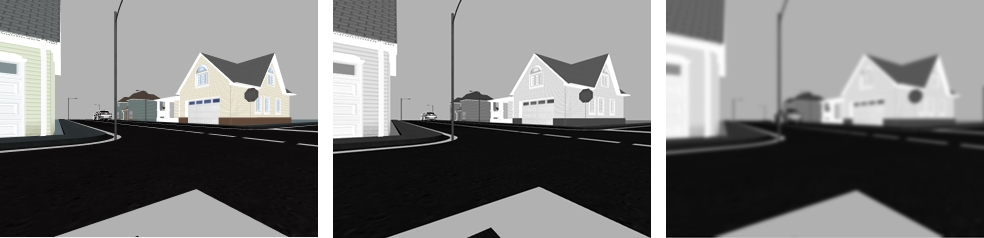
\includegraphics[width=1.0\textwidth]{figures/Stop/imgL.jpg}
		\caption{Imagen original, en escala de grises y suavizada}
		\label{fig.imgL}
		\end{center}
\end{figure}

\begin{figure}[H]
  \begin{center}
    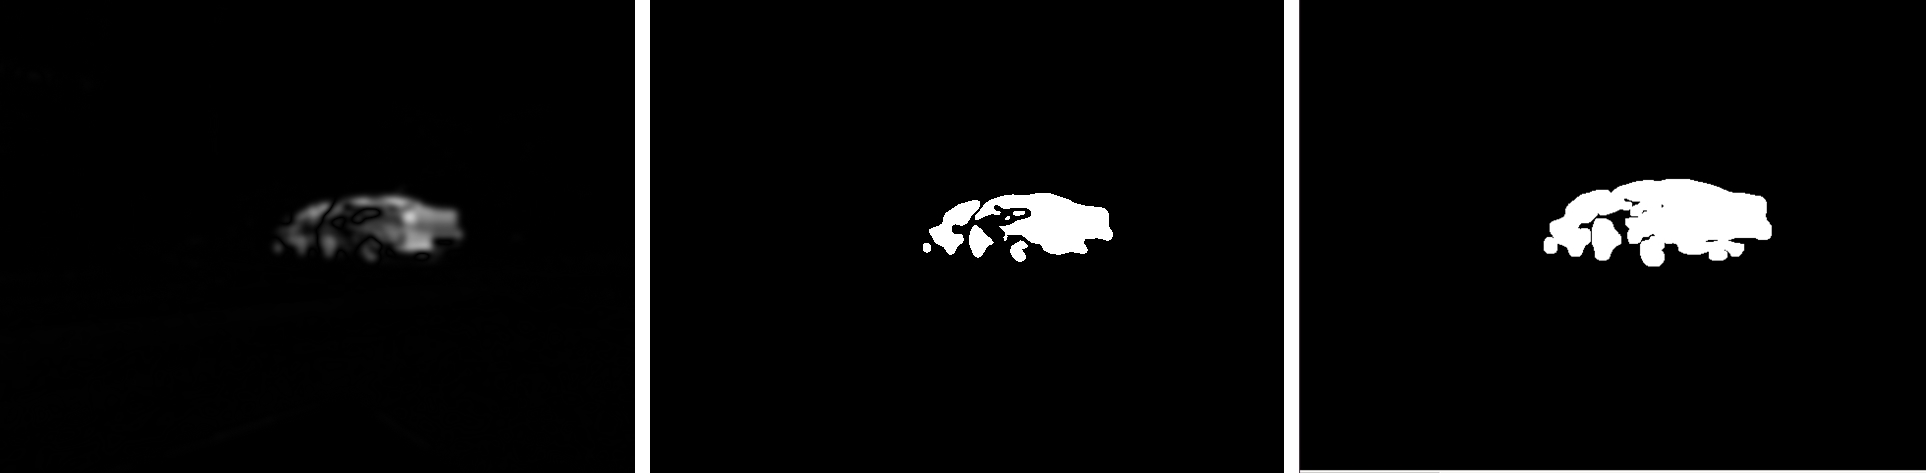
\includegraphics[width=1.0\textwidth]{figures/Stop/motionDetection.jpg}
		\caption{Proceso de detección de movimiento}
		\label{fig.motionDetection}
		\end{center}
\end{figure}

\subsection{Realización del giro}
Para decidir si el coche comienza o no a moverse de nuevo hemos creado la variable dinámica \textit{``detectionCar''}. Ésta irá disminuyendo su valor a lo largo del tiempo y aumentará si se detectan coches mediante la función \textit{``findCar''}. Cuando esta variable sea menor que el umbral establecido, el coche considerará que ha pasado un tiempo razonable sin detectar a otros vehículos y reanudará su ruta. \\

Ahora, el coche deberá girar a la izquierda o a la derecha. La dirección del giro se escogerá de manera aleatoria mediante la función creada \textit{chooseDir}. Una vez elegida la dirección el coche llevará a cabo un giro de 45º y después comenzará a detectar la carretera para situarse en el centro del carril derecho. Para realizar la detección de la carretera utilizaremos de nuevo la cámara situada en el techo del coche. A las imágenes captadas volveremos a aplicarles la función \textit{``filterHSV''} pero esta vez los valores del filtro serán los correspondientes al color gris de la carretera (Figura~\ref{fig.road}). Para seleccionar estos valores también utilizamos la herramienta ``colorTuner'' de JdeRobot.\\

\begin{figure}[H]
  \begin{center}
    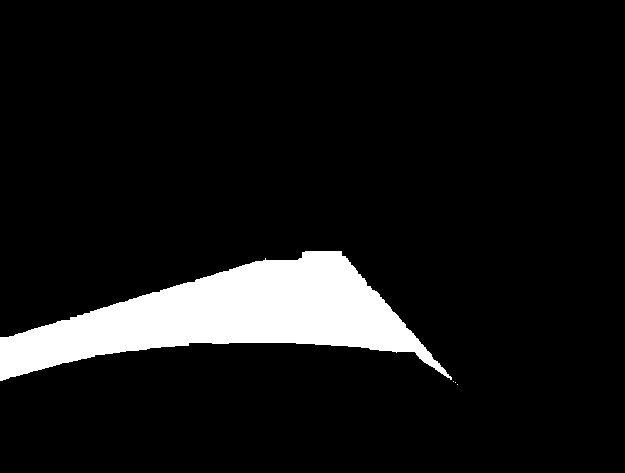
\includegraphics[width=0.5\textwidth]{figures/Stop/road.jpg}
		\caption{Carretera filtrada}
		\label{fig.road}
		\end{center}
\end{figure}

Una vez hemos realizado el filtrado de color de la imagen y hemos obtenido la carretera en primer plano, necesitamos hallar los límites de la carretera para que, posteriormente, el coche sea capaz de posicionarse correctamente en el carril derecho. Para ubicar los bordes, hemos creado la función \textit{``findRoad''} que recorrerá las columnas de la imagen y buscará los cambios de color que aparezcan en la fila 300 de la imagen. Hemos elegido esta fila para asegurar que contenga a la carretera (que estará en la parte inferior de la imagen). Si los píxeles cambian de negro a blanco se tratará del borde izquierdo y si cambian de blanco a negro se tratará del borde derecho. Después, deberemos encontrar la mitad de la carretera ya que marcará la separación de los dos carriles, y posteriormente, hallaremos la mitad del carril derecho (Figura~\ref{fig.desv}). Estas operaciones las llevará a cabo la función creada \textit{``findMidLane''}. \\

\begin{figure}[H]
  \begin{center}
    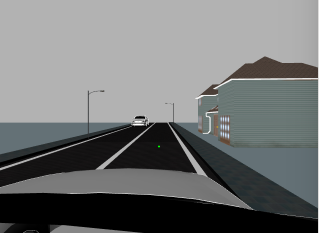
\includegraphics[width=0.5\textwidth]{figures/Stop/desv.png}
		\caption{Punto central del carril derecho de color verde}
		\label{fig.desv}
		\end{center}
\end{figure}

Para saber si el coche está circulando por el carril adecuado, haremos un control del pilotaje basándonos en la desviación que haya entre el centro de la imagen y el punto que marca el centro del carril derecho. Para ello, hemos creado la función \textit{``controlDesviation''} que aplicará una velocidad de giro a los motores directamente proporcional al valor de la desviación del vehículo en el carril por el que circula. También tendrá en cuenta el signo de la desviación ya que indica hacia qué lado se esta moviendo el coche. Si es negativa, se estará desviando hacia la derecha por lo que tendremos que corregir girando a la izquierda, y si es positiva, haremos el giro a la derecha. Si la desviación es pequeña, el coche simplemente irá recto sin girar.

\section{Experimentación}

\subsection{Ejecución típica} 
Para ejecutar esta práctica, es necesario abrir dos terminales y ejecutar los siguientes comandos:

\begin{enumerate}[1.]
\item Lanzar el simulador Gazebo:
	\begin{lstlisting}[frame=single]
		gazebo stop.world
	\end{lstlisting} 
	\begin{enumerate}[1b.]
	\item Se puede arrancar solo el simulador sin la interfaz gráfica:
		\begin{lstlisting}[frame=single]
		 	gzserver stop.world
		\end{lstlisting}
	\end{enumerate}
\end{enumerate}

\begin{enumerate}[2.]
\item	Ejecutar la práctica y lanzar la interfaz gráfica (\acrshort{gui}): 
	\begin{lstlisting}[frame=single]
		python2 stop.py -- --Ice.Config=stop.cfg
	\end{lstlisting} 
\end{enumerate}

En la Figura~\ref{fig.ejecucionFinal} se puede observar como, ejecutando el algoritmo explicado anteriormente, el coche es capaz de frenar cuando reconoce la señal de stop y después, en este caso, realizar el giro hacia la derecha. \\

\begin{figure}[H]
  \begin{center}
    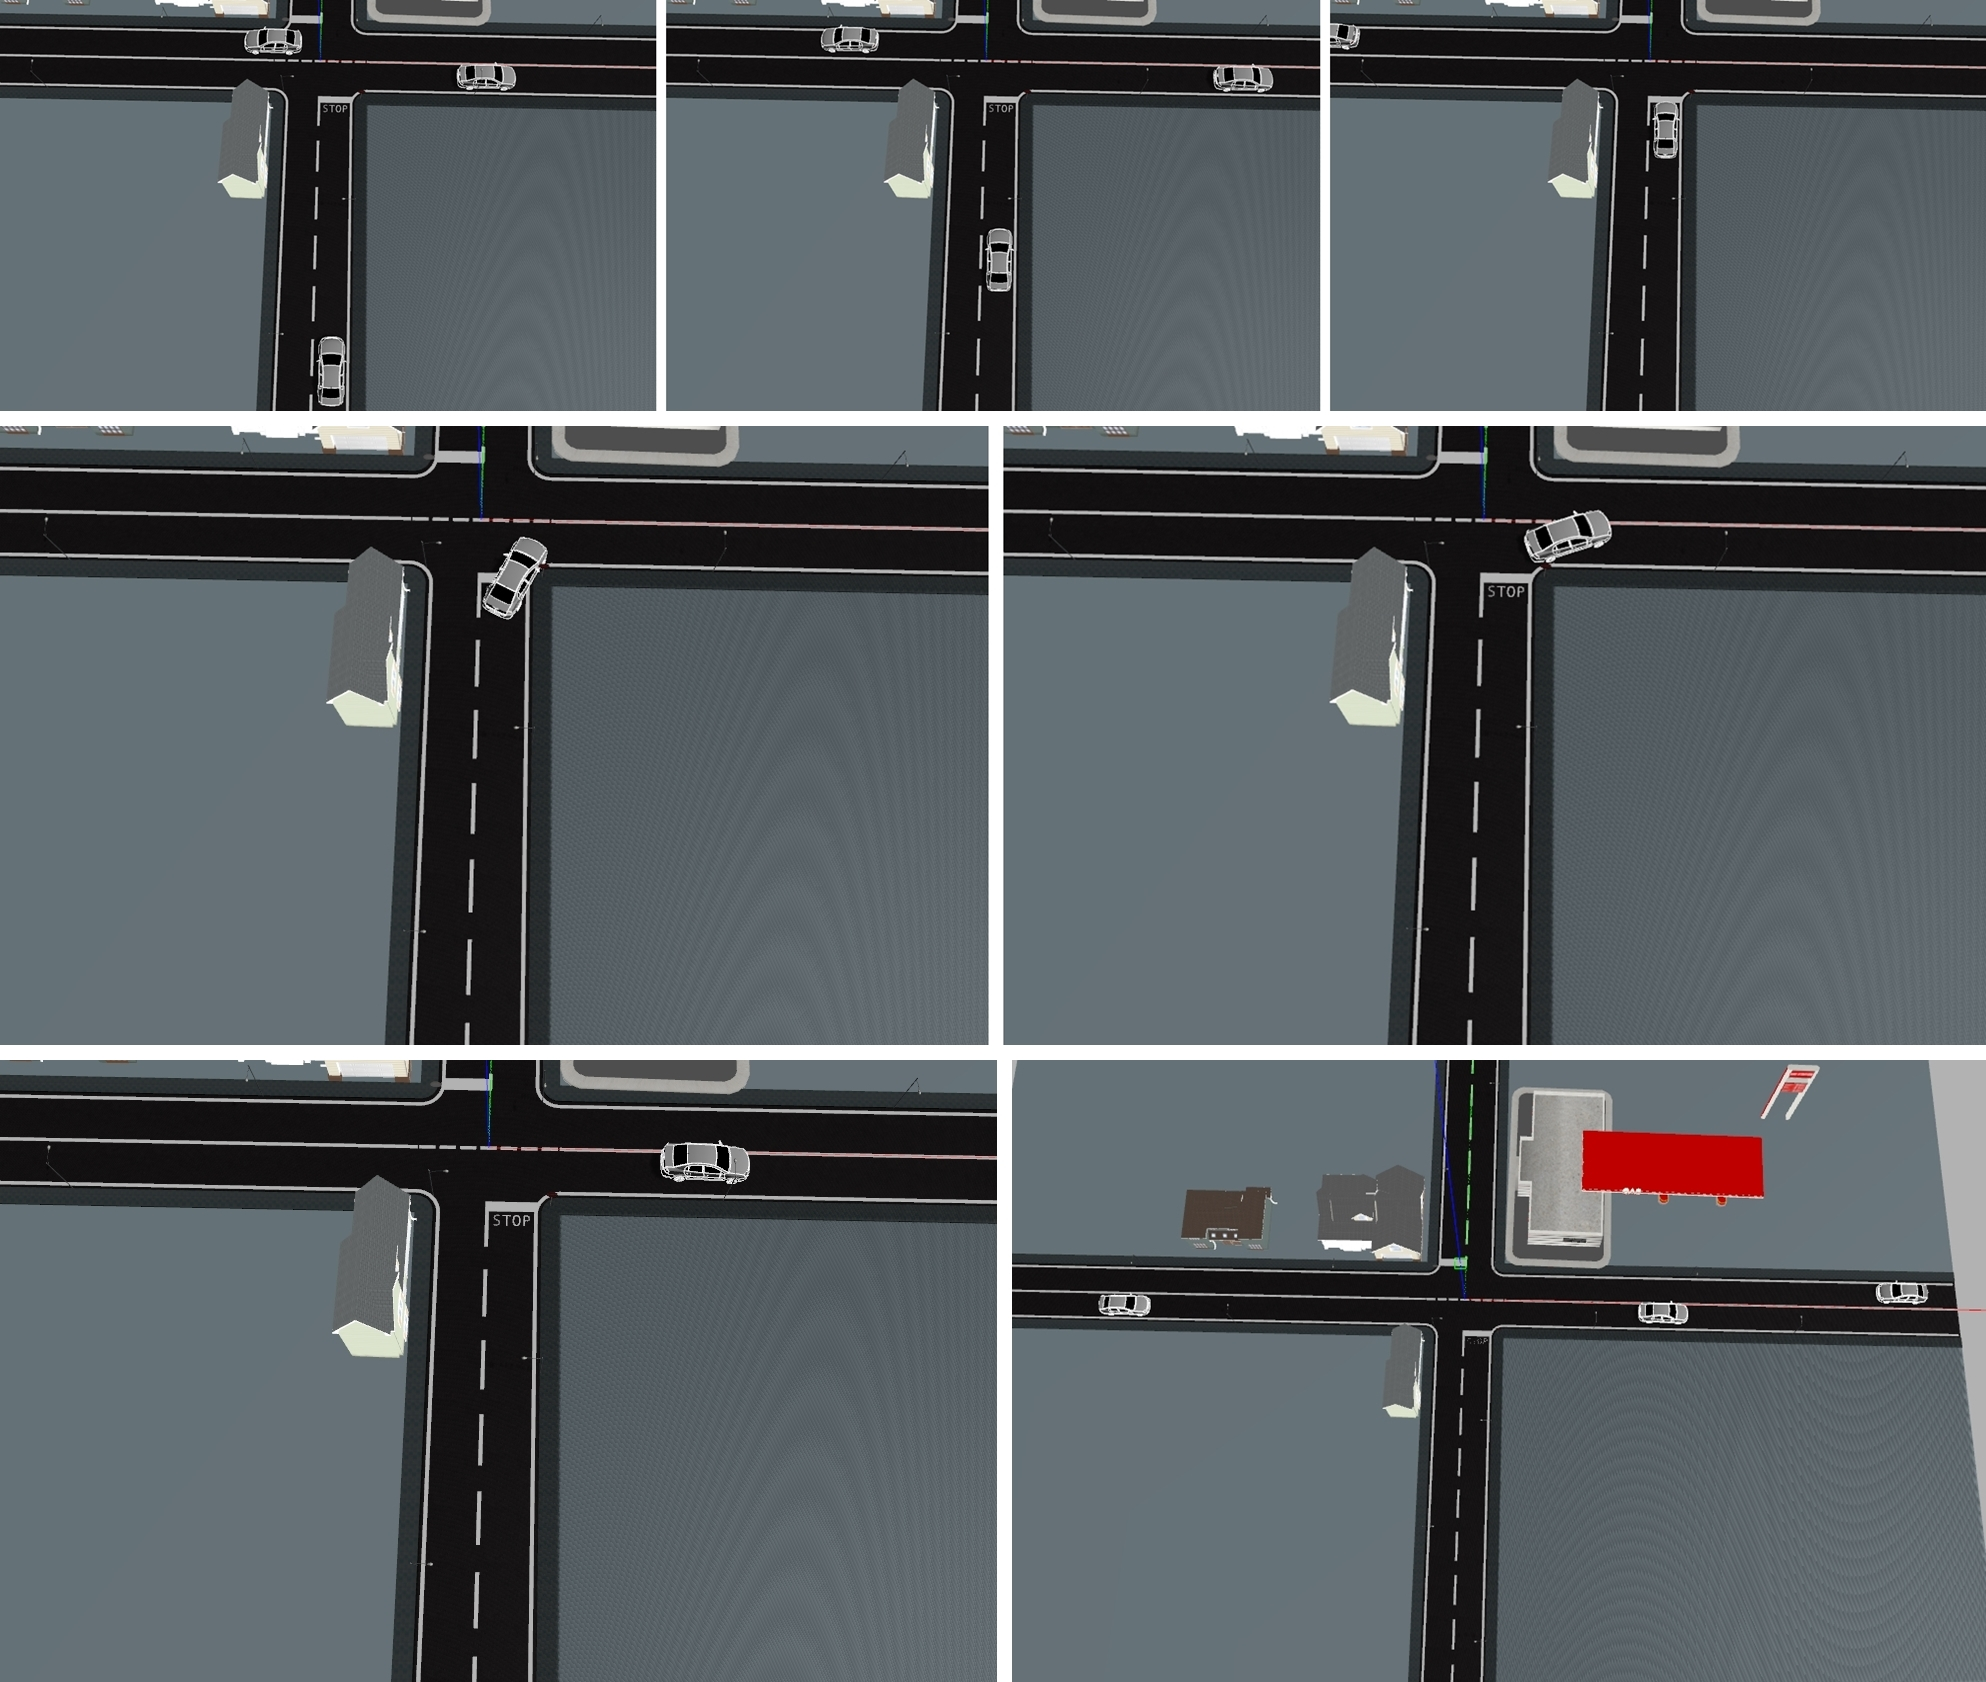
\includegraphics[width=0.9\textwidth]{figures/Stop/ejecucionFinal.jpg}
		\caption{Ejecución típica (giro a la derecha)}
		\label{fig.ejecucionFinal}
		\end{center}
\end{figure}


Una ejecución típica con el giro hacia la izquierda se puede ver en este vídeo \footnote{\url{https://www.youtube.com/watch?v=hF2i0rdlIqE}} y con el giro a la derecha en este otro \footnote{\url{https://www.youtube.com/watch?v=VXZtfHTGsW4}}.

\lhead[]{CAPÍTULO \thechapter. ASPIRADORA AUTÓNOMA}
\chapter{Práctica: Aspiradora autónoma (con autolocalización)}\label{cap.roomba}

\lhead[]{CAPÍTULO \thechapter. CONCLUSIONES}
\chapter{Conclusiones}\label{cap.conclusiones}
En este capítulo se comentarán las conclusiones que se han obtenido realizando este proyecto. También se expondrán posibles mejoras que aplicar a las distintas prácticas desarrolladas.

\section{Conclusiones}

Con la realización de este proyecto se ha cumplido el objetivo global de crear dos nuevas prácticas destinadas a la docencia de robótica en el entorno de JdeRobot Academy. El objetivo de dichas prácticas es conseguir que el estudiante que las realice adquiera conocimientos releacionados con la programación de diferentes robots.\\

Por cada práctica se ha desarrollado una infraestructura y un componente acádemico que simplifican la resolución del algoritmo permitiendo a los alumnos se abstriagan de problemas complejos que conlleva la práctica, tales como la programación de la interfaz gráfica o la comunicación con el simulador Gazebo, con los sensores y actuadores del robot. Además de la interfaz gráfica y el código auxiliar, se ha desarrollado una solución de refencia por práctica.\\

En primer lugar, se ha creado la práctica ``Reconocimiento de la señal stop''. Para esta práctica se ha creado un nuevo mundo en el simulador Gazebo que consiste, principalmente, en un cruce de carreteras donde se encuentra la señal de stop que hay que detectar. Además, también aparecen dos coches que se mueven automáticamente a lo largo de una de las carreteras. También se ha desarrollado una interfaz gráfica que permite ver las imágenes captadas por las cámaras instaladas en el coche, consiguiendo que resulte más sencillo el tratamiento digital de las imágenes. La solución de referencia elaborada consta de tres partes principales. La primera consiste en el reconocimiento de la señal de stop usando un filtro de color para detectar el color rojo y depués realizando una comparación con una plantilla de referencia para detectar la forma octogonal. En esta primera parte también se realiza el frenado del coche que  paulatinamente reduce la velocidad de manera proporcional al tamaño que tenga la señal de stop detectada. La segunda parte aborda la detección de otros coches mediante la detección de movimiento en las imágenes captadas. Por último, en la tercera parte, el coche realiza un giro a la izquierda o a la derecha (se elige de manera aleatoria) y, mediante el reconocimiento de la carretera, se sitúa en el centro del carril derecho.\\

En segundo lugar, se ha creado la práctica ``Aspiradora autónoma (con autolocalizción)''. Para esta práctica se ha modificado el mundo ``GrannyAnnie.world'', que consiste en una apartamento básico con distintas habitaciones y muebles. También se ha desarrollado una interfaz gráfica que muestra el mapa de la casa y marca las zonas por las que la aspiradora ha pasado, así como la orientación del robot. La solución llevada a cabo consta de dos partes principales: la planificación de la ruta y el pilotaje de la aspiradora. La planificación de la ruta está basada en un algoritmo de barrido de superficies en zigzag. Esta planificación utiliza el mapa de la casa para ir calculando las casillas a las que tiene que ir llegando la aspiradora. De esta manera, cada vez que la aspiradora llega a una nueva celda, se calcula la siguiente según si las casillas que rodean a la aspiradora (con vecindad a 4) son obstáculos, están libres o ya se ha pasado anteriormente por ese punto. Además, esta planificación calcula el punto al que retornar si la aspiradora no puede avanzar más. Para el pilotaje del robot se calcula la desviación que hay entre la aspiradora y la celda a la que tiene que dirigirse y según dicha desviación, aumentará o disminuirá su velocidad lineal y de giro. Para esta práctica también se ha creado un evaluador automático que, dependiendo del porcentaje recorrido de la casa, otorgará una nota final para el alumno.\\

A nivel presonal, hemos aprendido a manejar el simulador Gazebo, creando nuevos mundos y modelos, y a utilizar la plataforma JdeRobot para programar el comportamiento de diferentes robots autónomos. Uno de los elementos fundamentales de aprendizaje de esta plataforma es cómo se comunican los robots con los sensores y actuadores que poseen. Además, hemos aprendido a usar distintas bibliotecas de Python para poder desarrollar las prácticas. Al realizar este trabajo, también hemos comprendido como un problema de de gran envergadura se puede resolver dividiéndolo en objetivos más pequeños y a solucionar problemas típicos de ingeniería realizando dsitintas pruebas y experimentos para afinar el algoritmo (aplicando conocimientos adquiridos durante el grado o bien buscando y entendiendo nueva información).


\section{Trabajos futuros}
Como posibles mejoras a las prácticas y trabajos futuros relacionados con éstas, se proponen las siguientes opciones:

\begin{itemize}
\item Posibles trabajos y mejoras relacionadas con la práctica ``Reconocimiento de la señal stop'':

	\begin{itemize}
	\item Cuando se lleva a cabo el reconocimiento de la señal de stop se podría detectar, a parte del color rojo y la forma octogonal, la palabra 'STOP'. De este modo, el reconocimiento de la señal sería todavía más fiable.
	\item Utilizar otras técnicas de detección de movimiento más avanzadas para la detección de los coches como el uso de vectores de movimiento o el flujo óptico.
	\item Para disminuir el tiempo que el coche está parado en el cruce, se podría detectar el tamaño y el sentido de movimiento de los coches. De esta manera, si por ejemplo, se detectan coches pequeños significaría que éstos están lejos y que al coche le daría tiempo a realizar el giro en el cruce. Tembién si se detecta un coche por la cámara izquierda que se dirige hacia la izquierda, aunque sea grande, indica que el coche ya ha pasado el cruce y nuestro coche podría ir detrás sin chocarse.
	\item Se podría aumentar la dificultad de la práctica acelerando la velocidad e incrementando el número de los coches que circulan automáticamente por la carretera.
	\end{itemize}
	
\item Posibles trabajos y mejoras relacionadas con la práctica ``Aspiradora autónoma (con autolocalización)'':

	\begin{itemize}
	\item Durante la etapa de planificación de la ruta se podrían utilizar distintos tipos de algoritmos para el barrido de superficies. En vez de un recorrido en zigzag, se podría utilizar un recorrido en espiral. Al principio, la aspiradora iría al lado de la pared y realizaría la espiral hacia el interior de cada habitación. Seguiría guradando los puntos de retorno de la misma manera que en el zigzag y el punto crítico para comenzar una nueva espiral sería cuando la aspiradora tuviese todas las casillas que la rodean barridas o con obstáculos.
	\item No proporcionar el mapa de la casa para realizar el algoritmo de barrido. De esta manera, la aspiradora iría creando el mapa según su posición y los datos obtenidos por el sensor láser que tiene instalado.
	\item Optimizar el algoritmo de retorno para que encuantre la ruta más corta posible.
	\item Se podría probar el algoritmo creado en una aspiradora real. Así, se podría observar de manera exacta como funcionaría la solución realizada. Se pobaría en distintas habitaciones con diferentes obstáculos para lograr que el algoritmo fuera lo más robusto posible. 
	\end{itemize}
\end{itemize}


%https://programarfacil.com/blog/vision-artificial/deteccion-de-movimiento-con-opencv-python/

%%%%%%%%%%%%%%% Bibliograí­a %%%%%%%%%%%%%%%

%\nocite{*}
%\lhead[]{BIBLIOGRAFÍA}
%\bibliographystyle{unsrt}
\bibliography{Memoria}
\addcontentsline{toc}{chapter}{Bibliografía}

\end{document}